%%%%%%%%%%%%%%%%%%%%%%%%%%%%%%%%%%%%%%%%%%%%%%%%%%%%%%%%%%%%%%%%%%%%%%%%%%%%%%%%%%%%%
%%%%%%%%%          DOCUMENTO DE UNION DE CAPITULOS                      %%%%%%%%%%%%%
%%%%%%%%%%%%%%%%%%%%%%%%%%%%%%%%%%%%%%%%%%%%%%%%%%%%%%%%%%%%%%%%%%%%%%%%%%%%%%%%%%%%%
%\documentclass[12pt,oneside,a4paper]{book}
\documentclass[twoside,12pt, pdftex]{classes/CUEDthesisPSnPDF}
%{classes/CUEDthesisPSnPDF}

\usepackage{ae}
\usepackage[spanish]{babel}
\selectlanguage{spanish}
\usepackage[OT2,T1]{fontenc}
\usepackage{times}							%%% Uso de letra Time
\usepackage[utf8]{inputenc}				%%% Este paquete permite poner acentos directamente%%% 
\usepackage[pdftex]{graphicx,color}			%%% Inclusion de Figuras 
\usepackage{titlesec}
\usepackage{fancyhdr}
\usepackage{hyperref}
\usepackage{makeidx}
\usepackage{tocbibind} 
\usepackage[intlimits]{amsmath}
\usepackage{cancel}
\usepackage{listings}
\lstset{%			% Configuración de parámetros de listing.
basicstyle=\small\ttfamily,	% Códigos con fuente TrueType.
breaklines=true,		% Rompe líneas demasiado largas.
xrightmargin=1cm,		% Margen derecho.
escapeinside=wz,		% Para escapar a LaTeX.
}%
\usepackage[usenames,dvipsnames]{color}
\usepackage[final]{stylefiles/mcode}
\usepackage{enumerate}
\usepackage{wasysym}
\usepackage{caption}
\usepackage{graphicx}
\usepackage{subcaption}
\usepackage{booktabs}
\usepackage[toc,translate=babel]{glossaries}
\usepackage[gen]{eurosym}
%Macros:

%%%%%%%%%%%%%%% Formato de capítulos %%%%%%%%%%%%%%%%%%%%%
\newcommand{\sublinea}{\titlerule[.3mm] \vspace{.5mm} \titlerule[.75mm]}%
\titleformat{\chapter}[display] %%% definicion a cambiar % 
{\bfseries \sffamily \huge}%%% tipo de letra y tamao     % 
{\filleft                                                % 
 \LARGE \chaptertitlename\ %%% tamao Large               % 
 \Huge \thechapter}%%% n en Large                        % 
{3mm}%%% espacio entre etiqueta y cuerpo                 %
{\filleft}                                               %
[\vspace{0.5mm} \sublinea]                               % 
%%%%%%%%%%%%%%%%%%%%%%%%%%%%%%%%%%%%%%%%%%%%%%%%%%%%%%%%%%

%%%%%%%%%%%%%%% configuracin de pgina %%%%%%%%%%%%%%%%%%
\addtolength{\hoffset}{-5pt}                             %  
\addtolength{\voffset}{-25pt}                            %  
\addtolength{\textwidth}{50pt}                           %
\addtolength{\headheight}{12pt}                          % 
\addtolength{\textheight}{75pt}                          %  
%%%%%%%%%%%%%%%%%%%%%%%%%%%%%%%%%%%%%%%%%%%%%%%%%%%%%%%%%%

%%%%%%%%%%%%%%%%%%%%%%%%%%%%%%%%%%%%%%%%%%%%%%%%%%%%%%%%%%
%%%%%%%%%%%%%%%%% DEFINICIN DE MACROS %%%%%%%%%%%%%%%%%%%%
%%% MACRO FIGURA 										 %
%%%%%%%%%%%%%%%%%%%%%%%%%%%%%%%%%%%%%%%%%%%%%%%%%%%%%%%%%%
% Comando:                                               %
% \figura{nombre-fichero}{argumentos}{titulo}{etiqueta}  %
% argumnetos: width=Xcm,height=Ycm,angle=z               %  
%%%%%%%%%%%%%%%%%%%%%%%%%%%%%%%%%%%%%%%%%%%%%%%%%%%%%%%%%%
\newcommand{\figura}[4]{                                 %
   \begin{figure}[htbp]                                   %
   	\centering                                           %
	\includegraphics[#2]{#1}                             %
	\caption{\footnotesize#3}                            %
	\label{#4}                                           %
\end{figure}                                             %  
             }                                           %

%%%%%%%%%%%%%%%%%%%%%%%%%%%%%%%%%%%%%%%%%%%%%%%%%%%%%%%%%%

\newcommand{\figu}[4]{                                 %
   \begin{figure}[!hp]                                   %
	\centering                                           %
	\includegraphics[#2]{#1}                             %
	\caption{\footnotesize#3}                            %
	\label{#4}                                           %
\end{figure}                                             %  
             }                                           %
%%%%%%%%%%%%%%%%%%%%%%%%%%%%%%%%%%%%%%%%%%%%%%%%%%%%%%%%%%%
%%%%%%%%%%%%%%%%%%%%%%%%%%%%%%%%%%%%%%%%%%%%%%%%%%%%%%%%%%
% MACRO GRAD (Para colocar el simbolo ° ) % 
%%%%%%%%%%%%%%%%%%%%%%%%%%%%%%%%%%%%%%%%%%%%%%%%%%%%%%%%%%

\newcommand{\grad}{\hspace{-2mm}$\phantom{a}^{\circ}$\hspace{1mm}}

%%%%%%%%%%%%%%%%%%%%%%%%%%%%%%%%%%%%%%%%%%%%%%%%%%%%%%%%%%
% MACRO SUMARIO(SOLO PARA SER USADO DENTRO DE CAPITULOS) % 
%%%%%%%%%%%%%%%%%%%%%%%%%%%%%%%%%%%%%%%%%%%%%%%%%%%%%%%%%%
% Comando:                                               %
% \sumario{nombre de referencia de la seccin}            %
% ********** PARA SECCIONES ***************************  %     
%%%%%%%%%%%%%%%%%%%%%%%%%%%%%%%%%%%%%%%%%%%%%%%%%%%%%%%%%%
\newcommand{\sumario}[1]{                                %
\newline                                                 %
\vspace*{2pt}                                            %
\textsc{\ref{#1} $\circ$ \nameref{#1}}                   %
                          }                              %
%%%%%%%%%%%%%%%%%%%%%%%%%%%%%%%%%%%%%%%%%%%%%%%%%%%%%%%%%%
%%%%%%%%%%%%%%%%%%%%%%%%%%%%%%%%%%%%%%%%%%%%%%%%%%%%%%%%%%
% Comando:                                               %
% \subsumario{nombre de referencia de la subseccin}      %
% ********* PARA SUB-SECCIONES ************************* %
%%%%%%%%%%%%%%%%%%%%%%%%%%%%%%%%%%%%%%%%%%%%%%%%%%%%%%%%%%
\newcommand{\subsumario}[1]{                             %
\newline                                                 %
\vspace*{1pt}                                            %
\hspace*{1cm} {\small - \nameref{#1}}                    %
                          }                              %
%%%%%%%%%%%%%%%%%%%%%%%%%%%%%%%%%%%%%%%%%%%%%%%%%%%%%%%%%%
%%%%%%%%%%%%%%%%%%%%%%%%%%%%%%%%%%%%%%%%%%%%%%%%%%%%%%%%%%
% Comando:                                               %
% \subsumario{nombre de referencia de la subseccin}      %
% ********* PARA SUB-SUB-SECCIONES ********************* %
%%%%%%%%%%%%%%%%%%%%%%%%%%%%%%%%%%%%%%%%%%%%%%%%%%%%%%%%%%
\newcommand{\subsubsumario}[1]{                          %
\newline                                                 %
\vspace*{1pt}                                            %
\hspace*{2cm} {\small   \nameref{#1}}                    %
                          }                              %
%%%%%%%%%%%%%%%%%%%%%%%%%%%%%%%%%%%%%%%%%%%%%%%%%%%%%%%%%%
%%%%%%%%%%%%%%%%%%%%%%%%%%%%%%%%%%%%%%%%%%%%%%%%%%%%%%%%%%
% MACRO ECUACIN                                          % 
%%%%%%%%%%%%%%%%%%%%%%%%%%%%%%%%%%%%%%%%%%%%%%%%%%%%%%%%%%
% Comando:                                               %
% \ecu{etiqueta}{contenido}                              %
%%%%%%%%%%%%%%%%%%%%%%%%%%%%%%%%%%%%%%%%%%%%%%%%%%%%%%%%%%
\newcommand{\ecu}[2]{                                    %
  \begin{equation}                                       %
    #2                                      			 %
    \label{#1}                                           %
  \end{equation}           }                             %
%%%%%%%%%%%%%%%%%%%%%%%%%%%%%%%%%%%%%%%%%%%%%%%%%%%%%%%%%%
%%%%%%%%%%%%%%%%%%%%%%%%%%%%%%%%%%%%%%%%%%%%%%%%%%%%%%%%%%
% Referencia de Figura                                   % 
%%%%%%%%%%%%%%%%%%%%%%%%%%%%%%%%%%%%%%%%%%%%%%%%%%%%%%%%%%
% Comando:                                               %
% \reffig{nombre figura}                                 %
%%%%%%%%%%%%%%%%%%%%%%%%%%%%%%%%%%%%%%%%%%%%%%%%%%%%%%%%%%
\newcommand{\reffig}[1]{                                 %
  \textit{Figura \ref{fig:#1}}                           %
                        }                                %
%%%%%%%%%%%%%%%%%%%%%%%%%%%%%%%%%%%%%%%%%%%%%%%%%%%%%%%%%%
%%%%%%%%%%%%%%%%%%%%%%%%%%%%%%%%%%%%%%%%%%%%%%%%%%%%%%%%%%
% Referencia de anexo                                    % 
%%%%%%%%%%%%%%%%%%%%%%%%%%%%%%%%%%%%%%%%%%%%%%%%%%%%%%%%%%
% Comando:                                               %
% \refanex{nombre anexo}                                %
%%%%%%%%%%%%%%%%%%%%%%%%%%%%%%%%%%%%%%%%%%%%%%%%%%%%%%%%%%
\newcommand{\refanex}[1]{                                %
  \textit{Anexo \ref{#1}}			  			     %
}														 %
%%%%%%%%%%%%%%%%%%%%%%%%%%%%%%%%%%%%%%%%%%%%%%%%%%%%%%%%%%
%%%%%%%%%%%%%%%%%%%%%%%%%%%%%%%%%%%%%%%%%%%%%%%%%%%%%%%%%%
% Referencia de Seccion                                  % 
%%%%%%%%%%%%%%%%%%%%%%%%%%%%%%%%%%%%%%%%%%%%%%%%%%%%%%%%%%
% Comando:                                               %
% \refsec{nombre seccion}                                %
%%%%%%%%%%%%%%%%%%%%%%%%%%%%%%%%%%%%%%%%%%%%%%%%%%%%%%%%%%
\newcommand{\refsec}[1]{                                 %
  \textit{Secci\'on \ref{sec:#1}}						 %
}														 %
%%%%%%%%%%%%%%%%%%%%%%%%%%%%%%%%%%%%%%%%%%%%%%%%%%%%%%%%%%
%%%%%%%%%%%%%%%%%%%%%%%%%%%%%%%%%%%%%%%%%%%%%%%%%%%%%%%%%%
% Referencia de subseccion                               % 
%%%%%%%%%%%%%%%%%%%%%%%%%%%%%%%%%%%%%%%%%%%%%%%%%%%%%%%%%%
% Comando:                                               %
% \refsubsec{nombre subseccion}                          %
%%%%%%%%%%%%%%%%%%%%%%%%%%%%%%%%%%%%%%%%%%%%%%%%%%%%%%%%%%
\newcommand{\refsubsec}[1]{                              %
  \textit{Secci\'on \ref{subsec:#1}}                     %
                        }                                %
%%%%%%%%%%%%%%%%%%%%%%%%%%%%%%%%%%%%%%%%%%%%%%%%%%%%%%%%%%
% Referencia de Capitulo                                 % 
%%%%%%%%%%%%%%%%%%%%%%%%%%%%%%%%%%%%%%%%%%%%%%%%%%%%%%%%%%
% Comando:                                               %
% \refcap{nombre seccion}                                %
%%%%%%%%%%%%%%%%%%%%%%%%%%%%%%%%%%%%%%%%%%%%%%%%%%%%%%%%%%
\newcommand{\refcap}[1]{                                 %
  \textit{Cap\'itulo \ref{#1}}							 %
}														 %
%%%%%%%%%%%%%%%%%%%%%%%%%%%%%%%%%%%%%%%%%%%%%%%%%%%%%%%%%%
% Referencia de Ecuacin                                  % 
%%%%%%%%%%%%%%%%%%%%%%%%%%%%%%%%%%%%%%%%%%%%%%%%%%%%%%%%%%
% Comando:                                               %
% \refecu{nombre ecuaci\'on}                             %
%%%%%%%%%%%%%%%%%%%%%%%%%%%%%%%%%%%%%%%%%%%%%%%%%%%%%%%%%%
\newcommand{\refecu}[1]{                                 %
  \textit{Ec\hspace{1mm}\ref{#1}}                        %
                        }                                %
%%%%%%%%%%%%%%%%%%%%%%%%%%%%%%%%%%%%%%%%%%%%%%%%%%%%%%%%%%
%%%%%%%%%%%%%%%%%%%%%%%%%%%%%%%%%%%%%%%%%%%%%%%%%%%%%%%%%%
% Salto de renglon                                       % 
%%%%%%%%%%%%%%%%%%%%%%%%%%%%%%%%%%%%%%%%%%%%%%%%%%%%%%%%%%
% Comando:                                               %
% \salto                                                 %
%%%%%%%%%%%%%%%%%%%%%%%%%%%%%%%%%%%%%%%%%%%%%%%%%%%%%%%%%%
\newcommand{\salto}{                                     % 
\vspace*{11pt}      }                                    %
%%%%%%%%%%%%%%%%%%%%%%%%%%%%%%%%%%%%%%%%%%%%%%%%%%%%%%%%%%

%%%%%%%%%%%%%%%%%%%%%%%%%%%%%%%%%%%%%%%%%%%%%%%%%%%%%%%%%%
\newcommand{\referencia}[1]{                                  %
  \textit{[\cite{#1}]}                           %
                        }      							 %
%%%%%%%%%%%%%%%%%%%%%%%%%%%%%%%%%%%%%%%%%%%%%%%%%%%%%%%%%%

%%%%%%%%%%%%%%%%%%%%%%%%%%%%%%%%%%%%%%%%%%%%%%%%%%%%%%%%%%
% Unidades: Nanosegundos, micro metros, nanómetros, etc.
%
\newcommand{\ns} {\textrm{ns}}
\newcommand{\nanom} {\textrm{nm}}
\newcommand{\microm} {$\mu\textrm{m}$ }
\newcommand{\micromcuadrado} {$\mu\textrm{m}^2$}
\newcommand{\mmcuadrado} {$\textrm{mm}^2$}

%
%%%%%%%%%%%%%%%%%%%%%%%%%%%%%%%%%%%%%%%%%%%%%%%%%%%%%%%%%%

% Formato de las letras más cómodos.
\newcommand{\negrita}[1]{\textbf{#1}}
\newcommand{\cursi}[1]{\emph{#1}}
\newcommand{\layout}{\emph{layout }}
\newcommand{\netlist}{\emph{netlist }}

% Includes a MATLAB script.
% The first parameter is the label, which also is the name of the script
%   without the .m.
% The second parameter is the optional caption.
\newcommand{\matlabscript}[2]
  {\begin{itemize}\item[]\lstinputlisting[caption=#2,label=#1]{#1.m}\end{itemize}}

%Glosario:
\loadglsentries[main]{defns}
\makeglossaries

%\usepackage{cite}
\ifpdf
    \pdfinfo { /Title  (Diseño de un Sumador Rápido en tecnología CMOS submicrónica utilizando Herramientas de Software Libre)
               /Creator (TeX)
               /Producer (pdfTeX)
               /Author (Leandro Marsó)
               /CreationDate (D:20141106000000)  %format D:YYYYMMDDhhmmss
               /ModDate (D:20131014000000)
               /Subject (Diseño de Circuitos Integrados utilizando software libre)
               /Keywords (Circuitos Integrados VLSI Sumador Rápido)}
    
\fi

%\makeindex \label{indice}
\hyphenation{ GNU/Linux py-thon has-kell lay-out -net-list es-cla-re-ci-mien-to ma-te-ria-li-zar-se} 

% Para cambiar los nombres por defecto:
% Babel traducía table como cuadro. Yo lo cambio para tabla:
\addto\captionsspanish{%
  \renewcommand{\tablename}%
    {Tabla}%
}

\addto\captionsspanish{%
  \renewcommand{\listtablename}%
    {Índice de tablas}%
}

% Relacionado al paquete "glossaries".
\addto\captionsspanish{%
  \renewcommand*{\glossaryname}{Glosario}%
}





\begin{document}
\sloppy

\begin{titlepage}
\pagestyle{empty}       

\begin{center}
	\Huge{Universidad Nacional de Córdoba\\}
	\Large {Facultad de Ciencias Exáctas, Físicas y Naturales}\\

\vspace{1cm}

\includegraphics{tapa/escudo2.pdf}

\vspace{1cm}

	\Huge \textbf{\\[2ex]Proyecto Integrador de la Carrera Ingeniería Electrónica}
	\Large \textsl{\\[2ex] ''Diseño de un Sumador Rápido en tecnología CMOS submicrónica utilizando Herramientas de Software Libre''}

	\begin{normalsize}
	\end{normalsize}
	\begin{large}	
	\\ \textbf{Noviembre 2014}
	\end{large}

\end{center}

\vspace{0.5cm}

\begin{center}

\end{center}

% turn of those nasty overfull and underfull hboxes
\hbadness=10000
\hfuzz=50pt
\end{titlepage}
			%%% INCLUYE DE CARATULA 
\maketitle
%\frontmatter
%% Copyright 2007 by Till Tantau
%
% This file may be distributed and/or modified
%
% 1. under the LaTeX Project Public License and/or
% 2. under the GNU Public License.
%
% See the file doc/licenses/LICENSE for more details.



\documentclass{beamer}

%
% DO NOT USE THIS FILE AS A TEMPLATE FOR YOUR OWN TALKS�!!
%
% Use a file in the directory solutions instead.
% They are much better suited.
%


% Setup appearance:

\usetheme{Darmstadt}
\usefonttheme[onlylarge]{structurebold}
\setbeamerfont*{frametitle}{size=\normalsize,series=\bfseries}
\setbeamertemplate{navigation symbols}{}
\setbeamercovered{transparent}

% Standard packages

\usepackage[spanish]{babel}
\usepackage[latin1]{inputenc}
\usepackage{times}
\usepackage[T1]{fontenc}


% Setup TikZ

\usepackage{tikz}
\usetikzlibrary{arrows}
\tikzstyle{block}=[draw opacity=0.7,line width=1.4cm]


% Author, Title, etc.

\title[Dise�o de circuitos integrados con Software Libre]
{%
  Dise�o de un Sumador R�pido en tecnolog�a CMOS
  submicr�nica utilizando Herramientas de Software Libre
}

\author[Mars�]
{
  Leandro~Mars�\inst{1} \and
  Pablo~Cayuela~(Director)\inst{2} \and
  Hugo~Carrer~(Codirector)\inst{1} 
}

\institute[UNC and others]
{
  \inst{1}%
  Universidad Nacional de C�rdoba, Argentina
  \and
  \vskip-2mm
  \inst{2}%
  Universidad Tecnol�gica Nacional, FRC, Argentina
  \and
  \vskip-2mm
}

\date[FCEFyN 2006]
{Facultad de Ciencias Ex�ctas, F�sicas y Naturales, 2015}

% Delete this, if you do not want the table of contents to pop up at
% the beginning of each subsection:
\AtBeginSubsection[]
{
    \begin{frame}<beamer>{Temario}
          \tableofcontents[currentsection,currentsubsection]
	    \end{frame}
	  }

% The main document

\begin{document}

\begin{frame}
  \titlepage
\end{frame}

\begin{frame}{Temario}
  \tableofcontents
\end{frame}


\section{Introducci�n}
\subsection{Definiciones generales}
\begin{frame}{�Qu� es un sumador r�pido?}

\end{frame}
%-------------------------------------------------------------
\begin{frame}{�Qu� es un circuito integrado?}
  \begin{figure}
  \includegraphics[scale=0.30]{figuras/wafers.png}
  \caption{Obleas de silicio de 150, 200 y 300~mm de d�ametro, de un proceso CMOS.}
  \end{figure}
\end{frame}
%-------------------------------------------------------------
\begin{frame}{�Qu� es un circuito integrado?}
  \begin{figure}
  \includegraphics[scale=0.27]{figuras/encapsulado.png}
  \caption{Encapsulado del chip (a) y (b) una vista aumentada.}
  \end{figure}
\end{frame}
%-------------------------------------------------------------
\begin{frame}{�Qu� es un circuito integrado?}
  \begin{figure}
  \includegraphics[scale=0.45]{figuras/chips.png}
\caption{Algunos tipos de encapsulados comunes.}
  \end{figure}
\end{frame}
%-------------------------------------------------------------
\begin{frame}{�Qu� es un circuito integrado?}
  \begin{LARGE}
  \begin{center}
    \textbf{
  �Cu�nto podemos integrar?
}
\end{center}
\end{LARGE}

  \begin{columns}[t]
    \column{.43\textwidth}
    \begin{exampleblock}{CMOS 350~nm de AMS}
      18kGates/mm$^2$
    \end{exampleblock}
    \column{.43\textwidth}
    \begin{exampleblock}{CMOS 180~nm de AMS}
      118kGates/mm$^2$
\end{exampleblock}
    \end{columns}
\end{frame}


\begin{frame}{�Qu� es un circuito integrado?}
    \begin{table}[h]
      \centering
      \begin{tabular}{@{}lc@{}}
	\toprule
	Fabrica             & Proceso CMOS \\ \midrule
	TSMC                & 28~nm - 180~nm             \\
	Globalfoundries     & 14~nm - 180~nm             \\
	IBM                 & 32~nm -  250nm            \\
	ON Semi             & 0.35~um - 0.7~um           \\
	Austria Micro Systems & 180~nm - 0.35~um           \\ \bottomrule
      \end{tabular}
      \caption{Procesos disponibles por medio de MOSIS}
      \label{tab:procesosDisponibles}
    \end{table}
\end{frame}
%%-------------------------------------------------------------
\begin{frame}[label=libertades]{�Qu� es el Software Libre?}
\begin{definition}
  �Software libre� es el software que respeta la libertad de los usuarios y la comunidad. A grandes rasgos, significa que los usuarios tienen la libertad de ejecutar, copiar, distribuir, estudiar, modificar y mejorar el software. Es decir, el �software libre� es una cuesti�n de libertad, no de precio.
\end{definition}
\end{frame}
%-------------------------------------------------------------

\begin{frame}{Las cuatro libertades del Software Libre}
Un programa es software libre si los usuarios tienen las cuatro libertades esenciales:
\begin{itemize}
\item<1-> La libertad de ejecutar el programa como se desea, con cualquier prop�sito (libertad 0).
\item<2-> La libertad de estudiar c�mo funciona el programa, y cambiarlo para que haga lo que usted quiera (libertad 1). El \alert{acceso al c�digo fuente} es una condici�n necesaria para ello.
\item<3-> La libertad de redistribuir copias para ayudar a su pr�jimo (libertad 2).
\uncover{\item<4-> La libertad de distribuir copias de sus versiones modificadas a terceros (libertad 3). Esto le permite ofrecer a toda la comunidad la oportunidad de beneficiarse de las modificaciones. El \alert{acceso al c�digo fuente} es una condici�n necesaria para ello.
  }
\end{itemize}
\end{frame}

\begin{frame}{Las licencias de uso del software y su importancia}
  \begin{definition}
  Algo \alert{alerta} o no.

\end{definition}
  \hyperlink{libertades<2>}{\beamergotobutton{Cuatro libertades}}
  \hypertarget{return}{}


\end{frame}


\subsection{Planteamiento del problema y motivaci�n}

\begin{frame}{�C�mo dise�ar circuitos integrados con herramientas flexibles y accesibles para todo tipo de uso: acad�mico e industrial?}
  \begin{columns}[t]
    \column{.33\textwidth}
    \begin{exampleblock}{Econ�mico}
      $G\colon$
    \end{exampleblock}
    \column{.33\textwidth}
    \begin{exampleblock}{Acad�mico}
      $G\colon$
    \end{exampleblock}

    \column{.33\textwidth}
    \begin{exampleblock}{Genotype matrix}
      $G\colon$
    \end{exampleblock}
    \end{columns}

\end{frame}


\begin{frame}{What is haplotyping and why is it important?}
  You hopefully know this after the previous three talks\dots
\end{frame}

\begin{frame}[t]{General formalization of haplotyping.}
  \begin{block}{Inputs}
    \begin{itemize}
    \item A \alert{genotype matrix} $G$.
    \item The \alert{rows} of the matrix are \alert{taxa / individuals}.
    \item The \alert{columns} of the matrix are \alert{SNP sites /
        characters}. 
    \end{itemize}
  \end{block}
  \begin{block}{Outputs}
    \begin{itemize}
    \item A \alert{haplotype matrix} $H$.
    \item Pairs of rows in $H$ \alert{explain} the rows of $G$.
    \item The haplotypes in $H$ are \alert{biologically plausible}. 
    \end{itemize}
  \end{block}
\end{frame}


\begin{frame}[t]{Our formalization of haplotyping.}
  \begin{block}{Inputs}
    \begin{itemize}
    \item A genotype matrix $G$.
    \item The rows of the matrix are individuals / taxa.
    \item The columns of the matrix are SNP sites / characters.
    \item<alert@1->
      The problem is directed: one haplotype is known.
    \item<alert@1->
      The input is biallelic: there are only two homozygous
      states (0 and 1) and one heterozygous state (2).
    \end{itemize}
  \end{block}
  \begin{block}{Outputs}
    \begin{itemize}
    \item A haplotype matrix $H$.
    \item Pairs of rows in $H$ explain the rows of $G$.
    \item<alert@1> The haplotypes in $H$ form a perfect phylogeny.
    \end{itemize}
  \end{block}
\end{frame}


\begin{frame}{We can do perfect phylogeny haplotyping efficiently, but
    \dots}
  \begin{enumerate}
  \item \alert{Data may be missing.}
    \begin{itemize}
    \item This makes the problem NP-complete \dots
    \item \dots even for very restricted cases.
    \end{itemize}
    \textcolor{green!50!black}{Solutions:}
    \begin{itemize}
    \item Additional assumption like the rich data hypothesis. 
    \end{itemize}
  \item \alert{No perfect phylogeny is possible.}
    \begin{itemize}
    \item This can be caused by chromosomal crossing-over effects.
    \item This can be caused by incorrect data.
    \item This can be caused by multiple mutations at the same sites.
    \end{itemize}
    \textcolor{green!50!black}{Solutions:}
    \begin{itemize}
    \item Look for phylogenetic networks.
    \item Correct data.
    \item<alert@1->
       Find blocks where a perfect phylogeny is possible.
    \end{itemize}
  \end{enumerate}
\end{frame}



\begin{frame}{How blocks help in perfect phylogeny haplotyping.}
  \begin{enumerate}
  \item Partition the site set into overlapping contiguous blocks.
  \item Compute a perfect phylogeny for each block and combine them.
  \item Use dynamic programming for finding the partition.
  \end{enumerate}

  \begin{tikzpicture}
    \useasboundingbox (0,-1) rectangle (10,2);
    
    \draw[line width=2mm,dash pattern=on 1mm off 1mm]
      (0,1) -- (9.99,1) node[midway,above] {Genotype matrix}
      (0,0.6666) -- (9.99,0.6666)
      (0,0.3333) -- (9.99,0.3333)
      (0,0) -- (9.99,0) node[midway,below] {\only<1>{no perfect phylogeny}};

    \begin{scope}[xshift=-.5mm]
      \only<2->
      {
        \draw[red,block]            (0,.5)   -- (3,.5)
          node[midway,below] {perfect phylogeny};
      }
        
      \only<3->
      {
        \draw[green!50!black,block] (2.5,.5)   -- (7,.5)
          node[pos=0.6,below] {perfect phylogeny};
      }

      \only<4->
      {
        \draw[blue,block]           (6.5,.5) -- (10,.5)
          node[pos=0.6,below] {perfect phylogeny};
      }
    \end{scope}
  \end{tikzpicture}
\end{frame}

\begin{frame}{Objective of the integrated approach.}
  \begin{enumerate}
  \item Partition the site set into \alert{noncontiguous} blocks. 
  \item Compute a perfect phylogeny for each block and combine them. 
  \item<alert@1-> Compute partition while computing perfect
    phylogenies. 
  \end{enumerate}

  \begin{tikzpicture}
    \useasboundingbox (0,-1) rectangle (10,2);

    \draw[line width=2mm,dash pattern=on 1mm off 1mm]
      (0,1) -- (9.99,1) node[midway,above] {Genotype matrix}
      (0,0.6666) -- (9.99,0.6666)
      (0,0.3333) -- (9.99,0.3333)
      (0,0) -- (9.99,0) node[midway,below] {\only<1>{no perfect phylogeny}};

    \only<2->
    {
      \begin{scope}[xshift=-0.5mm]
        \draw[red,block] (0,.5)   -- (3,.5) 
          node[midway,below] {perfect phylogeny}
                         (8,.5) -- (9,.5);

        \draw[green!50!black,block]
          (3,.5)   -- (6,.5)
            node[pos=0.6,below] {perfect phylogeny}
          (6.4,.5)   -- (8,.5)
          (9,.5) -- (10,.5);

        \draw[blue,block] (6,.5) -- (6.4,.5)
          node[midway,below=5mm] {perfect phylogeny};
      \end{scope}
    }
  \end{tikzpicture}
\end{frame}


\begin{frame}{The formal computational problem.}

  We are interested in the computational complexity of \\
  \alert{the function \alert{$\chi_{\operatorname{PP}}$}}:
  \begin{itemize}
  \item It gets genotype matrices as input.
  \item It maps them to a number $k$.
  \item This number is minimal such that the sites can be
    covered by $k$ sets, each admitting a perfect phylogeny.
    \\
    (We call this a \alert{pp-partition}.)
  \end{itemize}
\end{frame}



\begin{frame}{Finding pp-partitions of haplotype matrices.}
  We start with a special case:
  \begin{itemize}
  \item The inputs $M$ are \alert{already haplotype matrices}.
  \item The inputs $M$ \alert{do not allow a perfect phylogeny}.
  \item What is $\chi_{\operatorname{PP}}(M)$?
  \end{itemize}
  \begin{example}
    \begin{columns}
      \column{.3\textwidth}
      $M\colon$
      \footnotesize
      \begin{tabular}{cccc}
        0 & 0 & 0 & 1 \\
        0 & 1 & 0 & 0 \\
        1 & 0 & 0 & 0 \\
        0 & 1 & 0 & 0 \\
        1 & 0 & 0 & 0 \\
        0 & 1 & 0 & 1 \\
        1 & 1 & 0 & 0 \\
        0 & 0 & 1 & 0 \\
        1 & 0 & 1 & 0
      \end{tabular}%
      \only<2>
      {%
        \begin{tikzpicture}
          \useasboundingbox (2.9,0);

          \draw [red, opacity=0.7,line width=1cm] (1.7 ,1.9) -- (1.7 ,-1.7);
          \draw [blue,opacity=0.7,line width=5mm] (0.85,1.9) -- (0.85,-1.7)
                                                  (2.55,1.9) -- (2.55,-1.7);
        \end{tikzpicture}
      }
      \column{.6\textwidth}
      \begin{overprint}
        \onslide<1>
        No perfect phylogeny is possible.
        
        \onslide<2>
        \textcolor{blue!70!bg}{Perfect phylogeny}
        
        \textcolor{red!70!bg}{Perfect phylogeny}
        
        $\chi_{\operatorname{PP}}(M) = 2$.
        
      \end{overprint}
    \end{columns}
  \end{example}
\end{frame}

\begin{frame}{Bad news about pp-partitions of haplotype matrices.}
  \begin{theorem}
    Finding \alert{optimal pp-partition of haplotype matrices}\\
    is equivalent to finding \alert{optimal graph colorings}.
  \end{theorem}

  \begin{proof}[Proof sketch for first direction]
    \begin{enumerate}
    \item Let $G$ be a graph.
    \item Build a matrix with a column for each vertex of $G$.
    \item For each edge of $G$ add four rows inducing\\the
      submatrix $\left(
        \begin{smallmatrix}
          0 & 0 \\
          0 & 1 \\
          1 & 0 \\
          1 & 1
        \end{smallmatrix}\right)$.
    \item The submatrix enforces that the columns lie in different
      perfect phylogenies. \qedhere  
    \end{enumerate}
  \end{proof}
\end{frame}

\begin{frame}{Implications for pp-partitions of haplotype matrices.}
  \begin{corollary}
    If $\chi_{\operatorname{PP}}(M) = 2$ for a haplotype matrix $M$,
    we can find an optimal pp-partition in polynomial time. 
  \end{corollary}

  \begin{corollary}
    Computing $\chi_{\operatorname{PP}}$ for haplotype matrices is
    \begin{itemize}
    \item $\operatorname{NP}$-hard,
    \item not fixed-parameter tractable, unless
      $\operatorname{P}=\operatorname{NP}$, 
    \item very hard to approximate.
    \end{itemize}
  \end{corollary}
\end{frame}

\subsection{Distintas arquitecturas de sumadores}


%\subsection{Hardness of PP-Partitioning of Genotype Matrices}


\begin{frame}{Finding pp-partitions of genotype matrices.}
  Now comes the general case:
  \begin{itemize}
  \item The inputs $M$ are \alert{genotype matrices}.
  \item The inputs $M$ \alert{do not allow a perfect phylogeny}.
  \item What is $\chi_{\operatorname{PP}}(M)$?
  \end{itemize}
  \begin{example}
    \begin{columns}
      \column{.3\textwidth}
      $M\colon$
      \footnotesize
      \begin{tabular}{cccc}
        2 & 2 & 2 & 2 \\
        1 & 0 & 0 & 0 \\
        0 & 0 & 0 & 1 \\
        0 & 0 & 1 & 0 \\
        0 & 2 & 2 & 0 \\
        1 & 1 & 0 & 0 
      \end{tabular}%
      \only<2>
      {%
        \begin{tikzpicture}
          \useasboundingbox (2.9,0);
          
          \draw [red, opacity=0.7,line width=1cm] (1.7 ,1.3) -- (1.7 ,-1.1);
          \draw [blue,opacity=0.7,line width=5mm] (0.85,1.3) -- (0.85,-1.1)
                                                  (2.55,1.3) -- (2.55,-1.1);
        \end{tikzpicture}
      }
      \column{.6\textwidth}
      \begin{overprint}
        \onslide<1>
        No perfect phylogeny is possible.
        
        \onslide<2>
        \textcolor{blue!70!bg}{Perfect phylogeny}
        
        \textcolor{red!70!bg}{Perfect phylogeny}
        
        $\chi_{\operatorname{PP}}(M) = 2$.
        
      \end{overprint}
    \end{columns}
  \end{example}
\end{frame}


\begin{frame}{Bad news about pp-partitions of haplotype matrices.}
  \begin{theorem}
    Finding \alert{optimal pp-partition of genotype matrices}
    is at least as hard as finding \alert{optimal colorings of
      3-uniform hypergraphs}. 
  \end{theorem}

  \begin{proof}[Proof sketch]
    \begin{enumerate}
    \item Let $G$ be a 3-uniform hypergraph.
    \item Build a matrix with a column for each vertex of $G$.
    \item For each hyperedge of $G$ add four rows inducing\\ the submatrix
      $\left(
        \begin{smallmatrix}
          2 & 2 & 2 \\
          1 & 0 & 0 \\
          0 & 1 & 0 \\
          0 & 0 & 1
        \end{smallmatrix}\right)
      $.
    \item The submatrix enforces that the three columns do not all lie
      in the same perfect phylogeny. \qedhere
    \end{enumerate}
  \end{proof}
\end{frame}

\begin{frame}{Implications for pp-partitions of genotype matrices.}
  \begin{corollary}
    Even if we know $\chi_{\operatorname{PP}}(M) = 2$ for a genotype matrix $M$,\\
    finding a pp-partition of any fixed size is still
    \begin{itemize}
    \item $\operatorname{NP}$-hard,
    \item not fixed-parameter tractable, unless
      $\operatorname{P}=\operatorname{NP}$, 
    \item very hard to approximate.
    \end{itemize}
  \end{corollary}
\end{frame}


\section{Implementaci�n}

\subsection{Dise�o digital}

\begin{frame}{Automatic optimal pp-partitioning is hopeless, but\dots}
  \begin{itemize}
  \item The hardness results are \alert{worst-case} results for\\
    \alert{highly artificial inputs}.
  \item \alert{Real biological data} might have special properties
    that make the problem \alert{tractable}.
  \item One such property is that perfect phylogenies are often
    perfect \alert{path} phylogenies:

    In HapMap data, in 70\% of the blocks where a perfect phylogeny
    is possible a perfect path phylogeny is also possible.
  \end{itemize}  
\end{frame}


\begin{frame}{Example of a perfect path phylogeny.}
  \begin{columns}[t]
    \column{.3\textwidth}
    \begin{exampleblock}{Genotype matrix}
      $G\colon$
      \begin{tabular}{ccc}
        A & B & C \\\hline
        2 & 2 & 2 \\
        0 & 2 & 0 \\
        2 & 0 & 0 \\
        0 & 2 & 2 
      \end{tabular}
    \end{exampleblock}

    \column{.3\textwidth}
    \begin{exampleblock}{Haplotype matrix}
      $H\colon$
      \begin{tabular}{ccc}
        A & B & C \\\hline
        1 & 0 & 0 \\
        0 & 1 & 1 \\
        0 & 0 & 0 \\
        0 & 1 & 0 \\
        0 & 0 & 0 \\
        1 & 0 & 0 \\
        0 & 0 & 0 \\
        0 & 1 & 1 
      \end{tabular}
    \end{exampleblock}

    \column{.4\textwidth}
    \begin{exampleblock}{Perfect path phylogeny}
      \begin{center}
        \begin{tikzpicture}[auto,thick]
          \tikzstyle{node}=%
          [%
            minimum size=10pt,%
            inner sep=0pt,%
            outer sep=0pt,%
            ball color=example text.fg,%
            circle%
          ]
        
          \node [node] {} [->]
            child {node [node] {} edge from parent node[swap]{A}}
            child {node [node] {}
              child {node [node] {} edge from parent node{C}}
              edge from parent node{B}
            };
        \end{tikzpicture}
      \end{center}
    \end{exampleblock}
  \end{columns}
\end{frame}


\begin{frame}{The modified formal computational problem.}
  We are interested in the computational complexity of \\
  the function $\chi_{\alert{\operatorname{PPP}}}$:
  \begin{itemize}
  \item It gets genotype matrices as input.
  \item It maps them to a number $k$.
  \item This number is minimal such that the sites can be
    covered by $k$ sets, each admitting a perfect \alert{path} phylogeny.
    \\
    (We call this a ppp-partition.)
  \end{itemize}
\end{frame}
%-------------------------------------------------------------

\subsection{Dise�o f�sico}
\begin{frame}{�rea}
  \begin{figure}
  \includegraphics[scale=0.450]{figuras/layout-disenos.pdf}
  \end{figure}
  \end{frame}
%-------------------------------------------------------------
\begin{frame}{Performance}
  \begin{figure}
  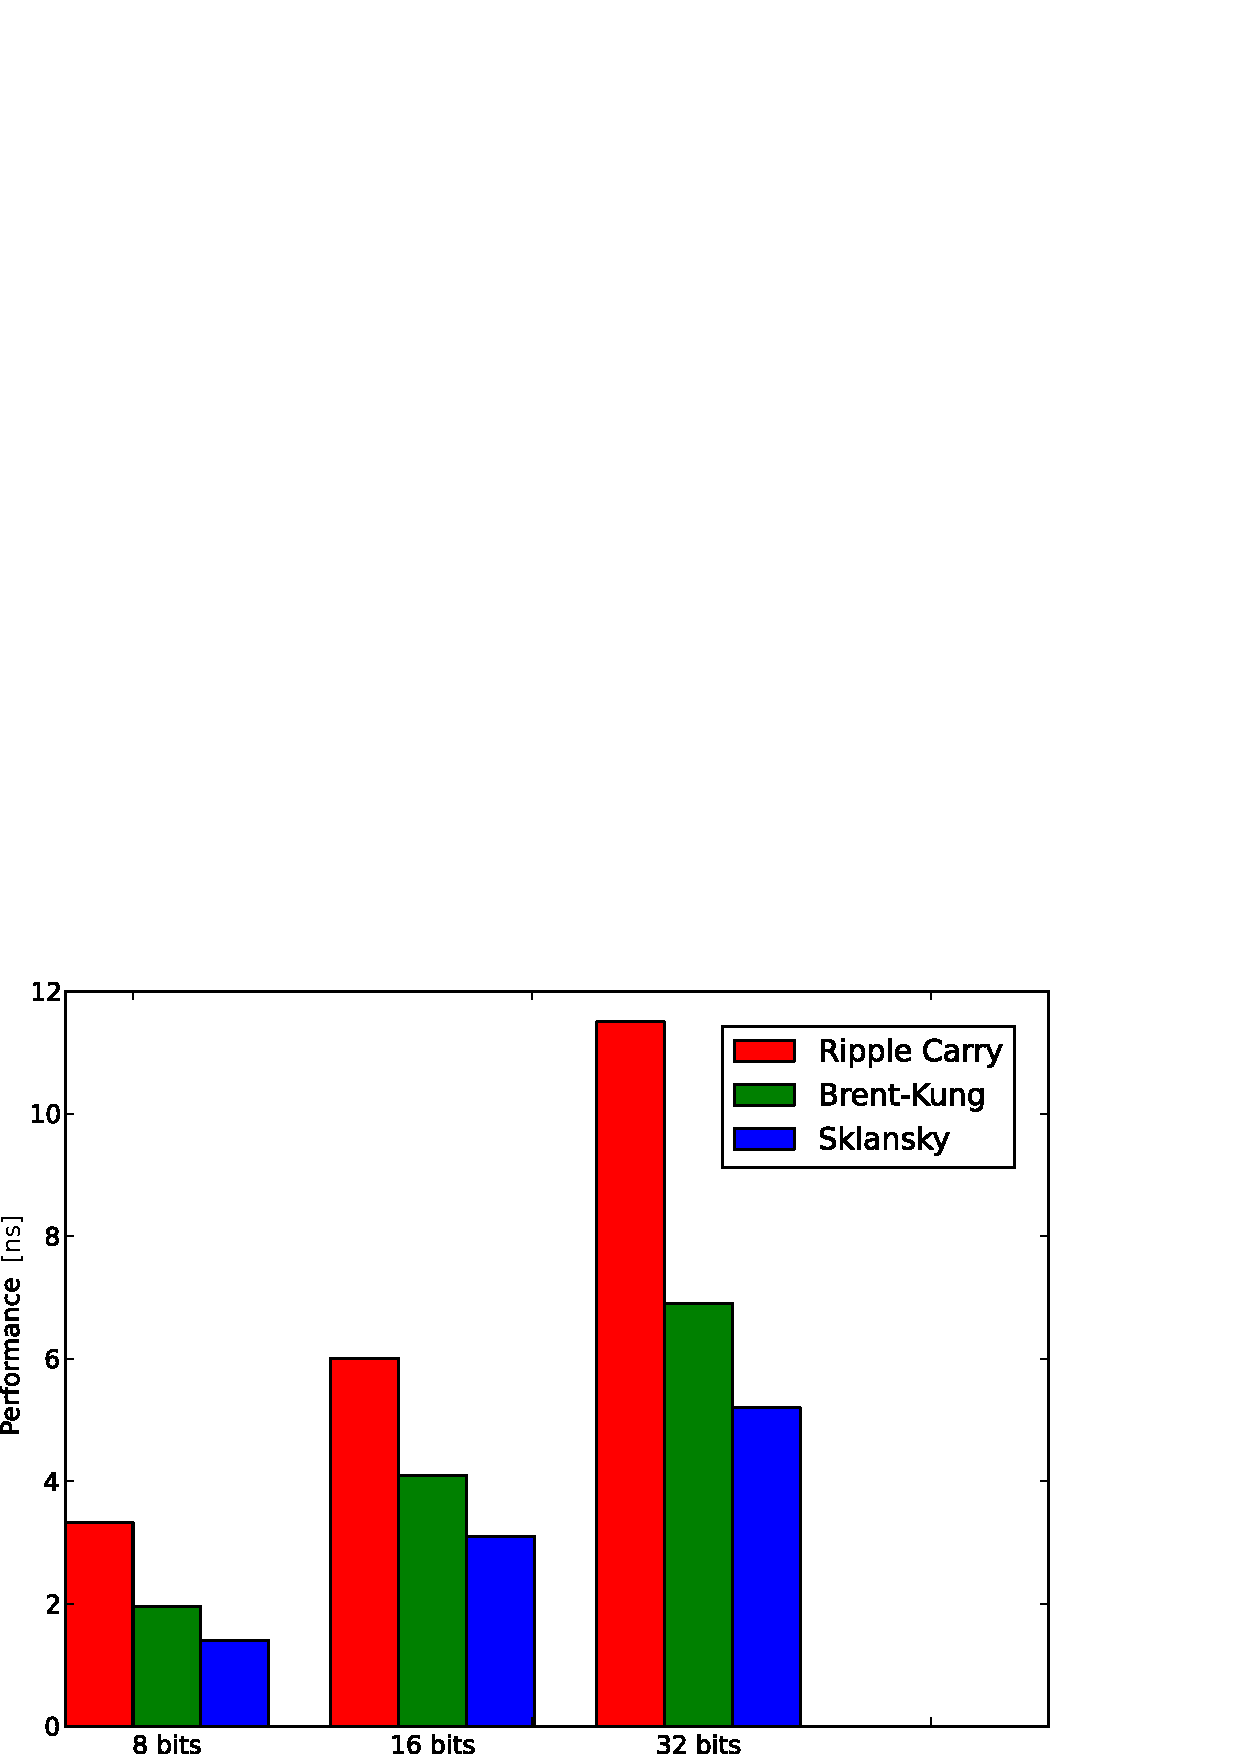
\includegraphics[scale=0.50]{figuras/barra_performance.pdf}
  \end{figure}
  \end{frame}
%-------------------------------------------------------------
\begin{frame}{Potencia}
  \begin{figure}
  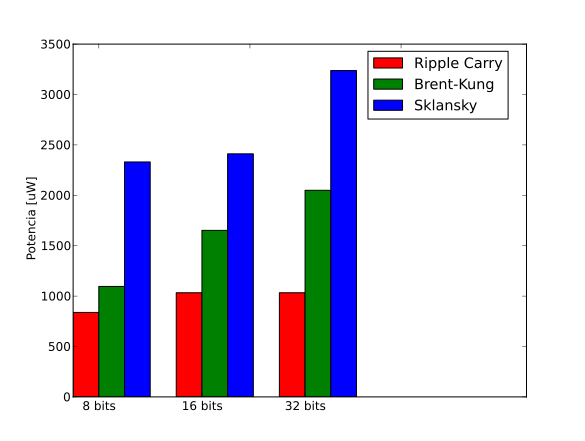
\includegraphics[scale=0.50]{figuras/barra_potencia2.pdf}
  \end{figure}
  \end{frame}
%-------------------------------------------------------------


\begin{frame}{Good news about ppp-partitions of genotype matrices.}
  \begin{theorem}
    \alert{Optimal ppp-partitions of genotype matrices} can be
    computed in \alert{polynomial time}. 
  \end{theorem}
  \begin{block}{Algorithm}
    \begin{enumerate}
    \item Build the following partial order:
      \begin{itemize}
      \item Can one column be above the other in a phylogeny?
      \item Can the columns be the two children of the root of a
        perfect path phylogeny?
      \end{itemize}
    \item Cover the partial order with as few compatible chain pairs 
      as possible. 

      For this, a maximal matching in a special graph needs to be
      computed.
    \end{enumerate}
  \end{block}
  \hyperlink{algorithm<1>}{\beamergotobutton{The algorithm in action}}
  \hypertarget{return}{}
\end{frame}

\section{Conclusiones}

\begin{frame}
  \frametitle<presentation>{Summary}

  \begin{itemize}
  \item
    Finding optimal pp-partitions is \alert{intractable}. 
  \item
    It is even intractable to find a pp-partition when \alert{just two 
      noncontiguous  blocks are known to suffice}.
  \item
    For perfect \alert{path} phylogenies, optimal partitions can be
    computed \alert{in polynomial time}.
  \end{itemize}
\end{frame}


\appendix
\section{Resumen}

\begin{frame}[label=algorithm]{The algorithm in action.}{Computation of
    the partial order.}
  \begin{columns}[t]
    \column{.4\textwidth}
    \begin{exampleblock}{Genotype matrix}
      $G\colon$
      \begin{tabular}{ccccc}
        A & B & C & D & E \\\hline
        2 & 2 & 2 & 2 & 2 \\
        0 & 1 & 2 & 1 & 0 \\
        1 & 0 & 0 & 1 & 2 \\
        0 & 2 & 2 & 0 & 0
      \end{tabular}
    \end{exampleblock}
    \column{.6\textwidth}
    \begin{exampleblock}{Partial order}
      \begin{tikzpicture}[node distance=15mm]
        \tikzstyle{every node}=
        [%
          fill=green!50!black!20,%
          draw=green!50!black,%
          minimum size=7mm,%
          circle,%
          thick%
        ]

        \node (A) {A};
        \node (B) [right of=A] {B};
        \node (C) [below of=B] {C};
        \node (D) [above of=A] {D};
        \node (E) [below of=A] {E};

        \path [thick,shorten >=1pt,-stealth'] (A) edge (E)
                         (B) edge (C)
                         (D) edge (A)
                             edge[bend right] (E);

        \uncover<2>{
        \path [-,blue,thick](A) edge (B)
                                edge (C)  
                            (B) edge (E)
                            (C) edge (E);}
      \end{tikzpicture}

      Partial order: \tikz[baseline] \draw[thick,-stealth'] (0pt,.5ex)
      -- (5mm,.5ex); 

      \uncover<2>{\textcolor{blue}{Compatible as children of root:
          \tikz[baseline] \draw[thick] (0pt,.5ex) -- (5mm,.5ex);}} 
    \end{exampleblock}
  \end{columns}  
\end{frame}

\begin{frame}{The algorithm in action.}{The matching in the special graph.}
  \begin{columns}[t]
    \column{.3\textwidth}
    \begin{exampleblock}{Partial order}
      \begin{tikzpicture}[node distance=15mm]
        \tikzstyle{every node}=%
        [%
          fill=green!50!black!20,%
          draw=green!50!black,%
          minimum size=8mm,%
          circle,%
          thick%
        ]

        \node (A)              {$A$};
        \node (B) [right of=A] {$B$};
        \node (C) [below of=B] {$C$};
        \node (D) [above of=A] {$D$};
        \node (E) [below of=A] {$E$};

        \path [thick,shorten >=1pt,-stealth'] (A) edge (E)
                         (B) edge (C)
                         (D) edge (A)
                             edge[bend right] (E);

        \path [-,blue,thick](A) edge (B)
                                edge (C)  
                            (B) edge (E)
                            (C) edge (E);

        \only<3->
        {
          \path[very thick,shorten >=1pt,-stealth',red] (D) edge (A) (B) edge (C);
          \path [-,red,very thick](E) edge (B);
        }
      \end{tikzpicture}
    \end{exampleblock}
    \column{.7\textwidth}
    \begin{exampleblock}{Matching graph}
      \begin{tikzpicture}[node distance=15mm]
        \tikzstyle{every node}=%
        [%
          fill=green!50!black!20,%
          draw=green!50!black,%
          minimum size=8mm,%
          circle,%
          thick,%
          inner sep=0pt%
        ]

        \node (A)              {$A$};
        \node (B) [right of=A] {$B$};
        \node (C) [below of=B] {$C$};
        \node (D) [above of=A] {$D$};
        \node (E) [below of=A] {$E$};

        \begin{scope}[xshift=4.75cm]
          \node (A')               {$A'$};
          \node (B') [right of=A'] {$B'$};
          \node (C') [below of=B'] {$C'$};
          \node (D') [above of=A'] {$D'$};
          \node (E') [below of=A'] {$E'$};
        \end{scope}
        
        \path [thick]    (A) edge (E')
                         (B) edge (C')
                         (D) edge (A')
                             edge (E');

        \path [blue,thick](A') edge (B')
                               edge (C')  
                          (B') edge (E')
                          (C') edge (E');

        \only<2->
        {
          \path[very thick,red] (D) edge (A')
                           (B) edge (C')
                           (B') edge (E');
        }
      \end{tikzpicture}
    \end{exampleblock}
  \end{columns}

  \medskip
  \uncover<2->{A \alert{maximal matching} in the matching graph
    \uncover<3>{induces\\ \alert{perfect path phylogenies}.}}

  \hfill\hyperlink{return}{\beamerreturnbutton{Return}}
\end{frame}

\end{document}



\begin{abstracts}
Aca escribo el resumen ...
\end{abstracts}

\pagenumbering{Roman}

\tableofcontents			%%% INCLUYE INDICE AL PRINCIPIO
\listoffigures 
\listoftables
\printglossaries

\chapter{ \textsc{ Introducción } }
\begin{abstract}
En el presente capítulo se describe en rasgos generales el flujo para el diseño de Circuitos Integrados de Aplicación Específica (\emph{ASIC} por su sigla en inglés), y la metodología utilizada para llevar adelante el diseño, implementación y tape out del mismo.
\end{abstract}
\section{Estructura del Proyecto Integrador}

\section{Planteamiento del problema y motivación}
El objetivo del trabajo es diseñar un sumador de n-bits, que pueda ser enviado a fabricar utilizando
procesos de fabricación CMOS para circuitos integrados. Integrar y documentar un flujo de diseño
de este sistema digital utilizando herramientas de Software Libre, será un subproducto de este
diseño, para lograr la base de conocimiento necesaria en el diseño de circuitos integrados con
tecnología CMOS. Este trabajo además de integrar todos los procesos de diseño de un Circuito
Integrado, pretende facilitar el acceso a las herramientas de diseño de circuitos integrados a los
estudiantes de grado.

\section{Objetivo}


\section{Plan de Trabajo}


\mainmatter

\part{Diseño Digital}\label{disenio_digital}
% Para compilar la primera vez que se agrega una referencia (/cite):
% Seguir estos cuatro pasos:
% latex Nombre-del-archivo.tex
% bibtex Nombre-del-archivo (sin el .tex)
% latex Nombre-del-archivo.tex
% latex Nombre-del-archivo.tex


% Etiquetas que uso para editar en la próxima iteración:
% FALTA, VER



%Escencia del tema.
%En cada capítulo empezar definiendo.
%En cada capitulo las referencias.

\chapter{ \textsc{ Especificaciones de diseño} }\label{chap:especificaciones}

\section{Introducción}\label{sec:intro_esp}
Los sumadores binarios son utilizados en la adición, la resta, la multiplicación y la división. La velocidad de un sistema de procesamiento de señales, o un sistema de comunicación depende fuertemente de \textbf{estas unidades funcionales\cite{rabaey2003}}. Para cada una de esas operaciones, son necesarios sumadores de distinta cantidad de bits en el mismo diseño. Por lo cual, no se trata solamente de encontrar la arquitectura que para una determinada cantidad de bits logre el mejor compromiso de área, potencia y velocidad. Sino que también esta relacion se mantenga óptima para diferentes tamaños del sumador. 

Por estas razones, precisamos diseñar un sumador de N-dígitos que sea lo más rápido posible, manteniendo una relación de compromiso óptima entre la velocidad, consumo de energía y área del circuito.
Estas características las resumimos en el cuadro \ref{cuadro:especifaciones}.
\begin{savenotes}
\begin{table}[h]
\centering
\begin{tabular}{@{}ll@{}}
\toprule
\textbf{Parámetro}  & \textbf{Especificación} \\ \midrule
Sumandos & Dos\footnote{Dejamos de lado las arquitecturas que implementan la suma de 3 o mas operandos, como pueden ser los sumadores Carry Save Adders} \\	
Cantidad de Dígitos & Parametrizable \\
Proceso de fabricación  & Disponible por medio de MOSIS\footnote{MOSIS es un servicio que permite la fabricación de Circuitos Integrados a muy bajo costo, por medio de obleas multiproyecto que pueden contener muchos diseños de distintos clientes} \\ 
Retardo de propagación  & Lo mas bajo posible                 \\
Potencia total disipada & Tan bajo como sea posible                 \\
Área del Circuito       & La menor posible                \\ \bottomrule
\end{tabular}
\caption{Especificaciones de diseño para el sumador binario}
\label{cuadro:especifaciones}
\end{table}
\end{savenotes}


\section{Métricas de calidad}
Definiremos las métricas que nos permitan dar cuenta de la calidad del diseño.
\subsection{Performance}

El término performance puede representar distintas métricas, según desde qué perpectiva se esté realizando el análisis. Pero si nos enfocamos puramente en el diseño, la performance en los sistemas síncronos se define usualmente\cite{rabaey2003} como la duración del período del reloj (o su frecuencia). El valor mínimo de período de clock que pueda ser usado para una tecnología y un diseño dado, está definido por múltiples factores, como el tiempo que le toma a las señales propagarse a través de la lógica (retardo de propagación), el tiempo que lleva entrar y salir los datos de los registros, la incertidumbre de llegada del reloj (\emph{clock uncertainty}). Pero el núcleo de todo análisis de performance reside en la performance de una sola compuerta.

\subsubsection{Retardo de propagación}
El retardo de propagación $t_p$ de una compuerta define cuán rápido responde un circuito a un cambio en su(s) entrada(s). Expresa el retardo experimentado por una señal cuando pasa a través de una compuerta. Medido entre el 50\% del punto de transición de entrada y salida, como mostramos en la figura \ref{fig:propagationDelay}, correspondiente al tiempo de propagación de una compuerta inversora. Ya que el tiempo de propagación es distinto según el flanco de entrada, se definen 2 tiempos de propagación. El $t_{pLH}$ es el tiempo de respuesta de una compuerta  para una transición de la salida desde bajo a alto, mientras que $t_{pHL}$ se refiere a el tiempo para una transición de la salida desde alto a bajo. El retardo de propagación $t_p$ se define como el promedio de estos dos.

$$ t_p = \frac{t_{pLH} + t_{pHL}}{2} $$

\subsubsection{Camino Crítico}
En un circuito digital con varias entradas y salidas, pueden existir mas de un camino desde la entrada hasta la salida. Se suele denominar camíno crítico a aquel camino que tenga el mayor retardo de propagación, ya sea por cantidad de lógica que atraviesa o por las capacidades parásitas de las conexiones. El retardo de propagación de este circuito será el retardo de propagación del camino crítico.


\begin{figure}[h]
\centering
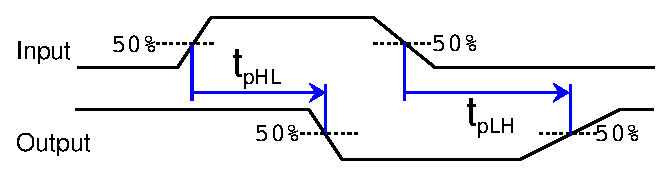
\includegraphics[scale=1.]{figuras/tiempo_retardo_tpHL-tpLH.eps}
  \caption{Retardo de propagación de un inversor}
  \label{fig:propagationDelay}
\end{figure}



\subsubsection{Mínimo retardo de propagación}

Para poder comparar la performance de distintas tecnologías, se busca un circuito que no incluya parámetros como el fan-in o fan-out, que influyen en los tiempos $t_f$, $t_r$ y $t_f$. Por ello, el circuito que es un estándar de facto para medir el tiempo de propagación, es el oscilador anillo (\emph{ring oscillator}), que es un número impar de inversores conectados en serie, con la salida conectada a la entrada. Este circuito oscilla espontaneamente, a una frecuencia de $T = 2 \times t_p \times N$, con $N$ el número de inversores en la cadena. 

Contar con esta métrica nos permitirá tener una referencia del límite inferior impuesto por la tecnología que se esté utilizando. Por ejemplo, tomemos la tecnología TSMC de 180~nm: La frecuencia de un oscilador anillo de 31 etapas es de 377,13~MHz. Es decir que el tiempo de propagación de una celda inversora en esta tecnología es $t_p = 47,8~ps$


%(TODO: Citar DIGITAL DESIGN OF SIGNAL PROCESSING SYSTEMS 5.5.1 )




%FIGURA
%(Multiplicadores, Filtros FIR, usando sumadores)


%Funcionamiento esperado: Se buscará acercarse lo mas posible a la frecuencia máxima de funcionamiento de los circuitos secuenciales para la tecnología CMOS seleccionada, que está caracterizada por la frecuencia de oscilación de un ring oscilator de 31 etapas. Lo
%mismo en cuanto a la especificación de potencia, se utilizará como referencia el número de unidad uW/MHz/gate de ese ring oscilator, que expresa la potencia de un inversor oscilando a la frecuencia máxima.




\subsection{Potencia promedio disipada}
Realizamos el análisis de potencia a lo largo de un período de tiempo $\mathrm{T}$. La potencia promedio disipada total la podemos calcular si conocemos la corriente instantánea que brinda la fuente de tensión $V_{DD}$, como podemos ver en la ecuación \ref{eq:pv}.
\begin{figure}[h]
\centering
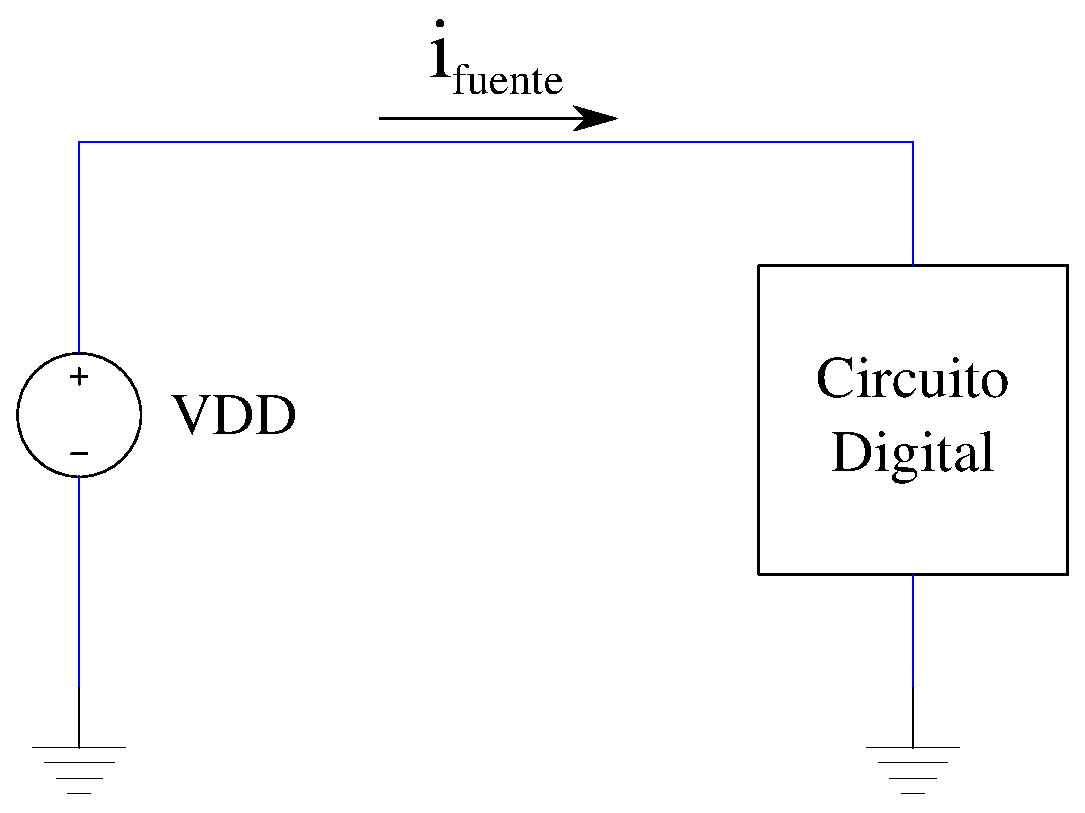
\includegraphics[scale=.5]{figuras/powerSupply.eps}
  \caption{Estimación de Potencia Promedio Disipada }
  \label{fig:powerSupply}
\end{figure}

\begin{equation}
P_{av} = \frac{1}{\mathrm{T}}\int\limits_0^T p(t)dt = \mathrm{\frac{V_{DD}}{T}}\int\limits_0^T i_{\mathrm{fuente}}(t)\mathrm{d}t 
\label{eq:pv}
\end{equation}
El período de tiempo que tomaremos para medir la potencia promedio lo elegiremos de forma tal que la medición resulte representativa del funcionamiento del circuito.

\subsection{Área}
La importancia de minimizar el área de los circuitos radica principalmente en que esta impacta fuertemente en el costo de cada \emph{die}\cite{HennessyPatterson}, ya que el costo es una función que depende de la cuarta potencia del área del circuito\cite{rabaey2003}. Además, los circuitos de menor área tienden a consumir menor energía. 


\subsection{Resumen}
A continuación resumimos en la tabla \ref{tabla:metricas} las métricas que utilizaremos para la comparación de las distintas arquitecturas de sumadores:
\begin{table}[h] 
\centering
\begin{tabular}{@{}ll@{}}
\toprule
\textbf{Métrica}  & \textbf{Unidades} \\ \midrule
Retardo de propagación & [ns] \\	
Potencia promedio disipada & [mW] \\
Área de circuito  & [$\mu\textrm{m}^2$] \\ \bottomrule
\end{tabular}
\caption{Métricas de comparación}
\label{tabla:metricas}
\end{table}




%Quality Metrics of a Digital Design
%Área 
%cost of die = f(die area)^4



%Background:
%Power consumption on cmos
%Dynamic Power, Static Power
%Delay in CMOS



%Glosario:

%Chip
%A tiny, thin square or rectangle that contains integrated
%electronic circuitry. Die are built in batches on wafers
%of silicon. A chip is a packaged die. Chips are also called
%processors and microprocessors. Microprocessors are the
%brains of computers, servers, communications products,
%and other digital devices

%Die: Alternate name for a chip, usually before it is packaged.
%See also Chip


%Wafer
%A thin silicon disc sliced from a cylindrical ingot. Used as
%the base material for building integrated circuits.

% Etiquetas que uso para editar en la próxima iteración:
% FALTA, VER


\chapter{ \textsc{ Diseño Digital } }\label{CONAMURI}

\textsl{ Bla bla bla bla bla bla bla ...\footnote{ Un groso } } 

%\vspace{10mm}

%\textbf{Por Magui Balbuena}\footnote{ Maguiorina (Magui) Balbuena  es dirigente de CONAMURI }

\vspace{10mm}

\section{Introducción}
Es importante lograr sumadores binarios rápidos y eficientes según el uso de área y potencial La suma es la operación elemental para lograr otras operaciones muy utilizadas en los circuitos aritméticos. Ejemplo de esto son los multiplicadores, la resta, división, los filtros FIR e IIR, por nombrar las más conocidas.

%FIGURA
%(Multiplicadores, Filtros FIR, usando sumadores)

Para cada una de esas operaciones, son necesarios sumadores de distinta cantidad de bits en el mismo diseño. Por lo cuál, no se trata solamente de encontrar la arquitectura que para una determinada cantidad de bits logre el mejor compromiso de área, potencia y velocidad. Sino también lograr una relación de compromiso según crece la cantidad de bits del sumador. 

\subsection{Semisumador y sumador completo}
\subsubsection{Semisumador}
El {\bf Semisumador} (Half-adder) recibe 2 bits de entradas \(a\) y \(b\) y produce un bit de suma \(s= a \oplus b\) y un bit de acarreo \(c= a b\).

\subsubsection{Sumador Completo}
Luego definimos un Sumador Completo de un bit, o Full Adder:
\begin{center}
\begin{tabular}{lll}
Entradas: & Bits de operandos \(a\) , \(b\) y carry-in \(c_{in}\) & (o \(x_i, y_i, c_i\) para la etapa \(i\)) \\
Salidas: & Suma \(s\) y carry-out \(c_{out}}\) & (o \(s_i\) y \(c_{i+1}\) para la etapa \(i\)) \\
\end{tabular}
\end{center}


\(s=x\oplus y \oplus c_{in}

%\(c_{out}= (a\wedge b )\vee (a \wedge c_{in}) \vee (b\wedge c_{in})\)

\(c_{out}= a b + a c_{in} + b c_{in}\)

Podemos construir un {\bf sumador completo} (full-adder) a partir del semisumador, como vemos en la siguiente figura:

\vspace{-1pt}

\begin{figure}[h]
  \centering
\begin{subfigure}[b]{0.3\textwidth}
                \centering
                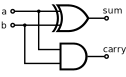
\includegraphics[width=\textwidth]{figuras/halfadd_schem.pdf}
                \caption{[Semisumador]}
                \label{fig:halfadder}
        \end{subfigure}
\begin{subfigure}[b]{0.3\textwidth}
                \centering
                \includegraphics[scale=0.95]{figuras/fullAdd.pdf}
                \caption{[Sumador completo]}
                \label{fig:fulladder}
        \end{subfigure}

  \caption{Bit adders}\label{fig:bitadders}

\end{figure}

\vspace{0.5cm}



\section{Selección de la arquitectura del sumador}

Proponemos el uso de Celdas estándard CMOS (Complementary Metal Oxide Silicon) para la implementación\footnote{Para ver otras posibilidades de implementación lógica, ver (FALTA CITA) RABAEY}. El carácter de nuestro flujo de diseño así lo requiere, ya que se utilizarán herramientas de síntesis de circuitos digitales basadas en celdas estándars. Quedan entonces descartadas las implementaciones utilizando transmition gates, lógica dinámica u otro tipo de implementacion lógica.

\subsection{Costo y Retardo de los circuitos combinacionales}
Cada circuito combinacional \(G\) tiene un costo y un retardo. El costo de un circuito combinacional es la suma de los costos de las compuertas en un circuito. Le asignamos un costo unitario a cada compuerta, y el costo del circuito combinacional \(c(G)\) es igual al número de compuertas en el circuito.

El retardo de un circuito combinacional \(d(G)\) se define igual al del retardo de una compuerta. Es el menor tiempo requerido para que las salidas se estabilicen, asumiendo que todas las entradas están estables. Para simplificar el análisis, se le asigna un retardo unitario a cada compuerta.



\subsection{Clasificación de los sumadores}

Dentro de los sumadores paralelos, se encuentran varias arquitecturas, cada una con sus ventajas y desventajas. Hacemos una lista de algunas de ellas:

\vspace{0.3cm}

\begin{tabular}{ |l|l| }
  \hline
  \multicolumn{2}{|c|}{Sumadores Binarios} \\
  \hline

RCA & Ripple Carry Adder \\
CLA & Carry Look-Ahead Adder \\
CSkA & Carry Skeep Adder \\
CA & Canonical Adders \\
BBCLA & Block-based Look-Ahead Adders \\
CondSumA & Conditional Sum Adder \\
CSeA & Carry Select Adder \\
HybAd & Hybrid Adders \\
NPA & Network Prefixs Adders: \\
& Ladner and Fischer \\
&Kogge-Stone \\
&Brent-Kung \\
&Skalansky \\
  \hline
\end{tabular}
\vspace{0.3cm}

%Carry Save Adder (CSaA) & \(O(n) \)& \(O(\log (n)) \)\\ \hline
%Carry Skip Adder (CSA) &\( O(n) \)& \(O(n^{l+2/l+1})\) \\ \hline
%Carry Increment Adder (CIA) &\( O(n)\) &\( O(n^{l+2/l+1})\) \\ \hline

\subsubsection{Ripple Carry Adder}

Definimos el sumador Ripple Carry Adder (RCA), utilizando \(n\) full-adders para sumar 2 operandos de \(n\) bits. El sumador de \(n\) bits produce una salida de \(n\) bits y una salida de acarreo \(c_{out}\)

Este sumador se implementa conectando como muestra la figura\ref{RCA} el bloque FA (Full Adder). El camino crítico de la señal se determina considerando el peor camino de propagación de la señal.  

%\vspace{-1pt}
\begin{figure}[h]
  \centering
%  \subfloat[Half adder]
{\label{RCA}\includegraphics[scale=1.5]{figuras/binnaryAdder.pdf}}
  \caption{Riple Carry Adder}
\vspace{-10pt}
\end{figure}

Resumimos las características y diferencias entre los distintos sumadores\cite{6120598}:
%\cite{estrada-gimenez}
%Comenzamos con el RCA (Ripple Carry Adder), que tiene un área O(n) y un retardo de compuerta (Delay) de O(n).
%Luego tenemos al CLA (Carry Look-Ahead Adder) con un área de O(n*log(n)) y un delay de O(log(n)).
%Carry Skip Adder(CSA)
%Carry Increment Adder (CIA) Área O(n) y Delay O (nl + 2/ l +1 )  
%Carry Select Adder (CSelA)Área O(n) y Delay O (nl + 2/ l +1 ) 
 
% El delay de un RCA está en pag. 77 de Computer Arithmetic de Behrooz Parhami


\subsubsection{Retardo Máximo y Área de las distintas arquitecturas}
\begin{table}[t]
\caption{Resumen Características de Sumadores}
\begin{tabular}{|l|l|l|}
\hline
\multicolumn{1}{|c|}{\textbf{Arquitectura}} & \multicolumn{1}{c|}{\textbf{Retardo Máx.   }} & \multicolumn{1}{c|}{\textbf{Área}} \\ \hline
Ripple Carry Adder (RCA) & \(O(n)\) & \(O(n)\) \\ \hline
Carry Save Adder (CSaA) & \(O(\log(n)) \)& \(O(n) \)\\ \hline
Carry Look-Ahead Adder (CLA) & \(O(\log(n))\) & \(O(n\log(n))\) \\ \hline
Carry Skip Adder (CSA) &\(O(n^{l+2/l+1})  \)& \(O(n)\) \\ \hline
Carry Increment Adder (CIA) &\(O(n^{l+2/l+1})  \)& \(O(n)\) \\ \hline
Carry Select Adder (CselA) &\(O(n^{l+2/l+1})  \)& \(O(n)\) \\ \hline
Ladner-Fisher &\( O(\log(n))\) & \(O(n\log(n))   \) \\ \hline
Skalansky &\( O(n\log_2(n))\) & \(O(\log^2(n))\) \\ \hline
Kogge-Stone & \( O(n\log_2(n))\) & \\ \hline
Han-Carlson &Falta &Falta \\ \hline 
Brent-Kung & \(O(\log_2(n))\ & \(O(n\log_2(n))\) \\ \hline

\end{tabular}
\label{sumadores}
\end{table}
%Agregar las referencias a los papers si se puede

%Para justificar la tabla de arriba, vemos los siguientes dos papers:

%"A unified Adder Design" - Wang, Parhi.

%CARACTERIZACIÓN DE SUMADORES EN TECNOLOGÍAS FUERTEMENTE SUBMICRÓNICAS -  Adrián Estrada, Carlos J. Jiménez, Manuel Valencia

\subsection{Carry Lookahead Adders}

La clave para sumar rápido es que el bloque generador de las señales de acarreo tenga baja latencia\cite{arithmeticComputer}.
%Pag. 85 - Section 5.6
ya que una vez que el acarreo en la posición \(i\) es conocido, se puede calcular la suma como:
$$s_i = a_i \oplus b_i\oplus c_i$$ 
%%Lo de arriba debe ser xor en vez de +


%$$(g,p) \circ (\hat{g},\hat{p}) = (g\vee(p\wedge\hat{g}),p\wedge\hat{g})$$

Con respecto al acarreo, lo importante es si en una posición dada el acarreo se \emph{genera} ó se \emph{propaga}. Con las siguientes ecuaciones lógicas podemos definir esas señales:
%

%\vee es el OR
%\wedge es el AND
%\oplus es el XOR
%$$g_i=a_i \wedge b_i$$
%$$p_i=a_i \oplus b_i$$
%$$a_i=\lnot{a_i}\wedge\lnot{b_i}=\lnot{(a_i \vee b_i)}$$
$$g_i=a_i  b_i$$
$$p_i=a_i \oplus b_i$$



Asumiendo que estas señales se han calculado y están disponibles, podemos calcular recursivamente el acarreo de la siguiente forma:
%$$c_{i+1}=g_i\vee (c_i \wedge p_i) $$
$$c_{i+1}=g_i + c_i p_i $$

Esto quiere decir que un acarreo entrará en una etapa \(i+1\) si este se genera en la etapa \(i\) ó entra en la etapa \(i\) y se propaga en esa etapa.

\subsection{Lower Bounds}
Teorema:
Si el número de entradas de cada compuerta combinacional está acotado por c, entonces para cada circuito combinacional \(G\) que implemente un \(sumador(n)\), se da que:

\(c(G) \greatereq n/c \) and \(d(G) \greatereq \log_{c}(n)\)

% INTERESANTE: Clock periods in contemporary microprocessors are rather short; they are shorter than 10 times the delay of a full-adder.





\subsection{Parallel Prefix Networks}
Se puede afirmar que los llamados sumadores paralelos prefijo son mejores con respecto al producto Potencia - Retardo. Aunque no hay una estructura que pueda calificarse como globalmente la mejor.

\subsection{Sumador Rápido de Brent-Kung}

Cuando se quiere tener en cuenta además del retardo y la potencia, el área de celdas e interconexión, se propone el sumador de Brent and Kung, ya que es una versión que considera el problema de la interconección entre las compuertas, de una forma que minimice el área, a costa de un aumento en el retardo.
%\cite{brent-kung}.

%FIGURA

%FALTA decir qué es el "l" de las funciones del área y delay.

%%% Bibliografia pa ver:

%[1] Digital arithmetic, Milos D. Ercegovac, and Thomas Lang, ed. Morgan and Kauffmann, 2004
% [2] Computer arithmetic algorithms, Israel Koren, ed. A.K. Peters. 2nd Edition, 2002
%[3] Circuitos integrados digitales, Jan M. Rabaey, Ananthan Chandrakasan, ad Borijove Nikolic, Prentice Hall, 2004.
% [4] A. Estrada Perez, “Metodología de caracterización de circuitos aritméticos para tecnologías submicronicas”, Trabajo de investigación del programa de doctorado Informática Industrial, Univ. de Sevilla, septiembre 2005.
%%%%%
%[6] Y. Choi, and E. E. Swartzlander, Jr, Parallel Prefix Adder Design with Matrix Representation, Proc. 17th IEEE Symposium on Computer Arithmetic, 2005, pp. 277-281.
%[7] S. Knowles, A Family of Adders, Proc. 15th IEEE Symposium on Computer Arithmetic, 2001, pp. 277-281

%[6] P. M. Kogge. Parallel Solutions of Recurrence problems, I.B.M. Journal Research and Development, March 1994.
%[7] P. M. Kogge and H. S. Stone, “A parallel Algorithm for the efficient solution of general class of recurrence equations”, IEEE Transaction Computers, vol V-22, No8, 1973, pp 786-793.
%[8] H. Ling, “High speed binary adders”, I. B. M. Journal Research and Develoment, vol 25, p.155-66, 1981.
%[9] T. D. Han, D. A. Carlson. “Fast area-efficient VLSI adder”, 8th Symposium on computer arithmetic, May 1987.
%[10] R. P. Brent and H. T. Kung, “A regular layout for parallel adders”, IEEE Tra

%p510 nikon


%Buscar Han - Carlson "Fast Area-efficient adders"

\chapter{\textsc{Implementación de los circuitos en lenguaje de descripción de hardware} }\label{implementaciónHDL}
\section{Introducción}
Utilizamos un lenguaje de descripción de \emph{hardware} (\gls{hdl} por su sigla en inglés) para implementar los distintos circuitos que evaluaremos, porque el problema planteado en el capítulo \ref{chap:especificaciones}, requiere que podamos crear un sumador de $n$ bits arbitrario, para lo cuál los HDL son la herramienta mas apropiada. Implementarlos por medio de esquemáticos llevaría mucho tiempo, por eso descartamos esa metodología. En cambio, cuando describimos un circuito con un HDL lo hacemos parametrizando el tamaño del mismo, y a la hora de simularlo o implementarlo físicamente, determinamos su tamaño y generamos automáticamente el circuito. 

\subsection{Breve reseña de los \gls{hdl}}
\gls{vhdl} y Verilog son los lenguajes más utilizados y conocidos para el diseño de circuitos integrados. \gls{vhdl} nace como lenguaje de documentación del comportamiento de los circuitos integrados de aplicación específica\footnote{Conocido comunente como \gls{asic}}. El departamento de defensa de Estados Unidos lo desarrolló para poder especificar a sus proveedores, cómo debía comportarse el sistema digital que les encargaba diseñar. Luego, surgio la idea de realizar una simulación lógica a partir de estos archivos \gls{vhdl}. Lo siguiente fué el desarrollo de herramientas de síntesis lógica a partir de estos archivos, para generar una implementación física del circuito. Con Verilog sucedió algo muy parecido, aunque dentro del ámbito de la industria. Por esta historia en común, se puede decir que estos dos lenguajes tienen varias finalidades, siendo la implementación en \emph{hardware} tan sólo una de ellas, es decir, uno puede describir circuitos que no son sintetizables. Por esa razón, y a pesar de ser los más utilizados y conocidos para describir circuitos digitales, no siempre son la mejor alternativa a elegir.

\subsection{Nuevos \gls{hdl}s}\label{subsec:nuevosHDL}
Podemos mencionar al menos tres lenguajes de descripción de \emph{hardware} que están siendo utilizados para el diseño de circuitos integrados, que nacieron con el objetivo de aprovechar las ventajas de nuevos lenguajes de programación, bajo el paradigma de la programación funcional. Estos son, \textbf{Lava}\cite{Lava} y \negrita{C$\lambda$aSH}\cite{Clash} basados en \textbf{Haskell}, y \textbf{Chisel}\cite{Chisel}, basado en \textbf{Scala}. En este tipos de lenguajes, un circuito que no sea sintetizable es un error de sintáxis. 

Otro lenguaje que queremos mencionar es \textbf{MyHDL}\cite{MyHDL}, un lenguaje basado en Python que brinda muchas ventajas de este lenguaje, que por estar basado en otro paradigma de programación, no lo agrupamos con los cuatro anteriores. Pero estos cinco lenguajes nos permiten:

\begin{itemize}
\item Usar un único lenguaje para describir (con distintos niveles de abstracción), simular, verificar e implementar el circuito.
\item Los circuitos se describen en Haskell, Scala o Python (según correspoda), el HDL es simplemente un conjunto de módulos que permiten realizar nuevas tareas relacionadas al diseño de \emph{hardware}, como puede ser crear un netlist \gls{vhdl}, simulación simbólica, etc. 
\item Generar automáticamente una descripción en \gls{vhdl} o Verilog, lo cuál nos permite utilizar herramientas de diseño físico que usan este tipo de lenguajes como entrada.
\item Describir circuitos que construimos a partir de subcircuitos, además de la posibilidad de reutilizar fácilmente patrones de conexión.
\end{itemize}

\subsection{¿Por qué Lava?}
Podemos elegir arbitrariamente cualquiera de estos lenguajes, ya que el circuito que lograremos es independiente del lenguaje utilizado. Por lo tanto, para este proyecto en particular\footnote{Es un circuito puramente combinacional} se puede elegir el HDL basado en el conocimiento y experiencia de uso en Haskell, Python o Scala.

Para describir el circuito, elegimos Lava. Quien haya utilizado alguna vez un lenguaje de programación funcional, entenderá fácilmente cómo describir circuitos. Quien no conozca este paradigma de programación, podrá aprender a utilizar Lava por medio de su documentación\cite{Lava-tutorial} sin muchas dificultades, ya que el paradigma de programación se basa en definir a los programas como se definen las funciones matemáticas. En Lava los circuitos son descriptos como funciones que operan sobre listas, tuplas o sobre circuitos. Esto último se debe a que el lenguaje Haskell permite la definición de funciones de alto orden, es decir podemos definir funciones que su dominio e imagen son funciones. 

Lava es simplemente un conjunto de módulos de Haskell, por lo tanto estamos unificando un conjunto de tareas del diseño digital utilizando un lenguaje de programación de propósito general. Las ventajas de este acercamiento al diseño son varias: 

\begin{itemize}
\item Disponibilidad de todas las librerías existentes en Haskell para ampliar las posibilidades de nuestra herramienta.
\item No se generan \cursi{bugs} típicos de implementar dos veces el mismo circuito en dos lenguajes de programación distintos: El primero en la implementación a nivel de sistema y el otro a nivel de \cursi{hardware}.
\item Se pueden aplicar técnicas de programación propias del lenguaje como \cursi{testing} o \cursi{model checking} con el circuito.
\item Permite manejar otros programas externos, por ejemplo lanzamos \negrita{minisat}\cite{minisat} para verificar formalmente nuestro circuito.  
\end{itemize}


Con la implementación del circuito utilizando este HDL, podemos generar un \negrita{netlist} \gls{vhdl}, hacer simulación digital, verificación formal de propiedades, y la ventaja de  


\section{Implementación en lenguaje de descripción de hardware}
Ya hemos presentado una descripción esquemática del sumador binario de \(n\) bits en la figura \ref{fig:RCA} y en la \ref{fig:bkungadder}. El objetivo es implementar estos circuito en Lava parametrizando el tamaño \(n\) de los sumandos. 

\subsection{Implementación del sumador de \textbf {ripple carry} en Lava}

\noindent Siguiendo la figura \ref{fig:halfadder}, definiremos el semisumador:
\begin{lstlisting}
halfAdd (a, b) = (s, c)
   where
      s = xor2 (a, b)
      c = and2 (a, b)
\end{lstlisting}
\noindent Para escribir el circuito del sumador completo usamos la figura \ref{fig:fulladder}, nombrando las señales internas y 
escribiendo los subcomponentes de la siguiente forma:
\begin{lstlisting}
fullAdd (cin, (a, b)) = (s, cout)
    where
       (sum1, carry1) = halfAdd (a, b)
       (s   , carry2) = halfAdd (cin, sum1)
       cout           = xor2 (carry2, carry1)
\end{lstlisting}

Por último escribimos la descripción del sumador binario (RCA) de la figura \ref{fig:RCA} de la siguiente forma:

\begin{lstlisting}
rcAdder (carryIn, ([], []))     = ([], carryIn)
rcAdder (carryIn, (a:as, b:bs)) = (sum:sums, carryOut)
   where
      (sum, carry)     = fullAdd (carryIn,(a, b))
      (sums, carryOut) = rcAdder (carry, (as, bs))
\end{lstlisting}

\subsection{Patrones de conexión}
\paragraph{Patrones de conexión estandars.} Los patrones de conexión son funciones de alto orden\footnote{Las funciones de alto orden (\emph{high order functions}) son funciones que toman otras funciones como argumento y devuelven otra función como resultado.} que pueden ser utilizadas para construir circuitos, les llamamos circuitos de alto orden o generadores de circuitos.

\begin{figure}[h]
  \centering
\hspace{-23pt}
%[width=\textwidth]
\begin{subfigure}[b]{0.45\textwidth}
                \centering
                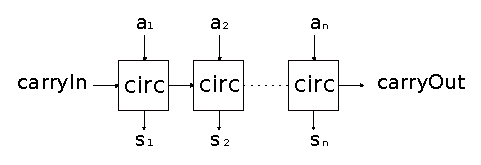
\includegraphics[scale=0.9]{figuras/rowCirc.eps}
                \caption{row}
                \label{fig:rowcirc}
        \end{subfigure}
\begin{subfigure}[b]{0.25\textwidth}
                \centering
                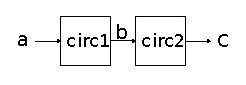
\includegraphics[scale=1]{figuras/serial.eps}
                \caption{serial}
                \label{fig:serial}
        \end{subfigure}
\begin{subfigure}[b]{0.30\textwidth}
                \centering
                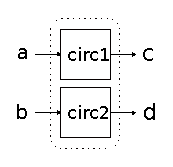
\includegraphics[scale=1]{figuras/par.eps}
                \caption{parallel}
                \label{fig:parallel}
        \end{subfigure}
  \caption{Diferentes patrones de conexión de circuitos}\label{fig:pattern}
\end{figure}


Observando la definición de {\footnotesize\verb|rcAdder|} y su topología, podemos generalizar esa estructura de conexión reemplazando el circuito por un parámetro, que en la definición\footnote{Esto es posible dado que Haskell implementa \emph{pattern matching}.} del circuito será una entrada mas. A ese parámetro lo nombramos {\footnotesize\verb|circ|}:

\begin{lstlisting}
row circ (carryIn, ([])) = ([], carryIn)
row circ (carryIn, a:as) = (b:bs, carryOut)
   where
      (b, carry)     = circ (carryIn, a)
      (bs, carryOut) = row circ (carry, as)
\end{lstlisting}

La función {\footnotesize\verb|row|} toma un circuito {\footnotesize\verb|circ|}, un conjunto de entradas, y las conecta como se muestra en la figura \ref{fig:rowcirc}. Ahora, usando el generador de circuito {\footnotesize\verb|row|}, el sumador binario lo podemos describir mas simplemente asi:
{\footnotesize
\begin{verbatim}
rcAdder' (carry, inps) = row fullAdd (carry, inps)
\end{verbatim}
}
Inclusive para simplificar mas, podemos currificar\footnote{Currificar, es una referencia al lógico Haskell Curry, y hace referencia a la técnica que consiste en transformar una función que utiliza una n-tupla como argumento, en una función que utiliza un único argumento.} la definición:
{\footnotesize
\begin{verbatim}
rcAdder'' = row fullAdd
\end{verbatim}
}

Definir {\footnotesize\verb|rcAdder'|} y {\footnotesize\verb|rcAdder''|} de esa forma es bastante conveniente ya que podemos pensar en término de \emph{generadores de circuitos} en vez de recursión sobre listas.

Ya que hemos visto la ventaja de definir los patrones de conexión, presentamos dos generadores de circuitos que vamos a usar mas tarde:

{\footnotesize
\begin{verbatim}
par cir1 cir2 (a, b) = (c, d)
   where
      c = cir1 a
      d = cir2 b
\end{verbatim}
}
Es muy útil definir una versión mas gráfica de la función {\footnotesize\verb|par|}, si definimos el operador infijo {\footnotesize \verb1-|-1}:
{\footnotesize
\begin{verbatim}
cir1 -|- cir2 = par cir1 cir2 
\end{verbatim}
}
Y por último la conexión serie y su versión con el operador infijo:
{\footnotesize
\begin{verbatim}
serial cir1 cir2 a = c
   where
      b = cir1 a
      c = cir2 b
\end{verbatim}
}
{\footnotesize
\begin{verbatim}
cir1 ->- cir2 = serial cir1 cir2
\end{verbatim}
}
\subsection{Sumador de Brent-Kung}
\subsubsection {Operador de Brent-Kung}
\noindent Comencemos a describir el sumador de Brent-Kung.
En Lava, podemos describir el circuito que implementa la función \ref{gap} siguiendo la figura \ref{dotOp}:

\begin{lstlisting}
dotOp ((g1, p1) ,(g, p)) = (go, po)
   where
      go = or2 (g, and2 (p, g1))
      po = and2 (p, p1)
\end{lstlisting}

\subsubsection {Generación y Propagación del Acarreo}
\noindent En Lava escribimos asi lo que captamos de la figura \ref{gAndPs}:
\lstset{language=Haskell}
{
\begin{lstlisting}
gAndPs ([],[]) = []
gAndPs (a:as, b:bs) = (g,p):gps
   where
      (g, p) = (and2 (a, b),xor2 (a, b))
      gps    = gAndPs (as, bs)
\end{lstlisting}
}


Para ver una explicación con mayor nivel de detalles de cómo construir el circuito, ver el manual de Lava \cite{Lava-tutorial} en conjunto con el paper aqui citado \cite{4638988}


\subsubsection {Red de Prefijos Paralelos para el sumador de Brent-Kung}
\noindent Ahora para describir esta red que usamos en la figura \ref{fig:bkungadder} y mostramos un ejemplo de una red para 16 bits en a figura \ref{bKung16}, nos basamos en un patrón recursivo que propone Sheeran \cite{Shee07} al que le llama \emph{wrap}. En cada paso de la iteración tomamos el resultado anterior (el circuito \(P\)) y le aplicamos el operador punto antes y después de forma intercalada como se puede ver en la figura \ref{sheeranrecurrence}. Esto nos lleva a construir redes como la de la figura \ref{bKung16}.


\begin{figure}[h!]
\centering
 \begin{subfigure}{0.4\textwidth}
    \centering
    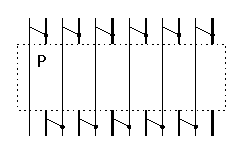
\includegraphics[scale=2.2]{figuras/sheeranrecurrence.eps}
%\vspace{0.05cm}
    \caption{Patrón de recurrencia}
    \label{sheeranrecurrence}
 \end{subfigure}
 \begin{subfigure}{0.5\textwidth}
    \centering
    \includegraphics[scale=1.92]{figuras/wrapR.eps}
    \caption{Primeras iteraciones de ppNet}
    \label{firstsiter}
 \end{subfigure}
 \caption{Construcción de la red de prefijos paralelos de Brent-Kung.}
\end{figure}


La figura \ref{firstsiter} representa las dos primeras iteraciones del circuito \verb|ppNet|, en el cual la caja de lineas punteada es el caso base de la descripción, los puntos negros son la función \verb|dotOp|. Lo que producimos con esta función recursiva son redes como la de la figura \ref{bKung16}.

A continuación, describimos el circuito \verb|ppNet|, pero antes escribimos las funciones auxiliares \verb|dop|, \verb|unzipl|, \verb|zipl|, \verb|comb|, \verb|posComb|, \verb|miti| y \verb|wrap|, que nos servirán para escribir \verb|ppNet|:


%abss era abs, pero lo renombré xq latex lo resaltaba como una función.
\begin{lstlisting}
dop [a, b] = [a, dotOp(a, b)]
--
unzipl []        = ([],[])
unzipl [a]       = ([a], [])
unzipl (a:b:abss) = (a:as, b:bs)
   where
      (as, bs) = unzipl abss
--
zipl ([], [])     = []
zipl ([a], [])    = []
zipl (a:as, b:bs) = a:b:zipl(as, bs)
--
-- La forma en que hemos escrito las funciones zipl y unzipl 
-- son la clave para lograr una descripcion de un sumador 
-- binario que acepte cualquier cantidad de entradas
--
comb []     = []
comb [a]    = []
comb (a:as) = dop [a, head as] ++ comb (tail as)
--
posComb (a:as)  = a: (comb (init as))++ [last as]
--
miti p = unzipl ->- (id -|- p) ->- zipl
--
wrap p = comb ->- miti p ->- posComb 
\end{lstlisting}

\noindent Luego finalemente, podemos describir {\verb|ppNet|}:

\begin{lstlisting}
ppNet [a]    = []
ppNet [a, b] = dop [a, b]
ppNet as     = wrap ppNet as
\end{lstlisting}


\subsubsection{Circuito top level}
Ahora que ya tenemos construidas todas las partes del sumador, sólo resta juntarlas siguiendo el esquemático de la figura \ref{fig:bkungadder}. Prestar atención a que el circuito \verb|fork| realiza una copia de las señales, el \verb|even| deja pasar los bits pares, \verb|odd| los impares, \verb|id| es la función identidad y \verb|sums| mapea los bits de entrada con la función booleana XOR, salvo el primer y último bit:

\begin{lstlisting}
fork as = (as, as)
--
even as = cs
   where
      (bs,cs) = unzip as
--
odd as = bs
   where
      (bs,cs) = unzip as
-- Unas definiciones mas cortas:
dropP = id -|- odds
dropG = even -|- ppNet
--
sums (a:as,bs) = (a:lastXor (as,init bs),cOut)
   where
      cOut = last bs
--
lastXor (as, bs) = map xor2 cs
   where
      cs = zipp (as, bs)
--
zipp ([],[]) = []

zipp (a:as, b:bs) = c:cs  -- da lo mismo que poner (c:cs)
   where
      c  = (a, b)
      cs = zipp (as, bs)
\end{lstlisting}

\noindent Y el circuito completo es:
\begin{lstlisting}
fastAdd = gAndPs ->- fork ->- dropG ->- dropP ->- sums
\end{lstlisting}


\subsection{Sumador de Sklansky}
En el apéndice \ref{chap:sklansky-lava} brindamos la descripción en Lava del sumador.


\subsection{Simulación}
En Lava podemos simular el circuito usando la operación {\footnotesize\verb.simulate.}, el circuito y el estado de las entradas, por ejemplo:

{\footnotesize
\begin{verbatim}
simulate fastAdd ([high,low],[low,high])
\end{verbatim}
}

\noindent devuelve:{\footnotesize \verb|([high,high],low)|}. También podemos simular secuencia de entradas con la operación {\footnotesize\verb|simulateSeq|}:

{\footnotesize
\begin{verbatim} 
simulateSeq halfAdd [(low,low),(high,low),(low,high)]
\end{verbatim}
}

\noindent que devuelve {\footnotesize\verb|[(low,low),(high,low),(high,low)]|}

\subsubsection{Simulaciones con números enteros en base diez}
Lava nos permite una interfase con números enteros, por si nos interesa simular utilizando esta representación numérica en vez de la binaria. Esto lo logramos si definimos una función como la siguiente, que toma dos enteros y convierte el segundo en un número binario de la cantidad de bits que indica el primero:
\begin{lstlisting}
int2bin 0 num = []

int2bin n num = (bit:bits)
  where
    (bit, num_) = numBreak num
     bits      = int2bin (n-1) num_
\end{lstlisting}

\subsubsection{Método de validación del hardware}
Para este diseño en particular, no utilizaremos la simulación como una forma de validar el correcto funcionamiento del circuito, por eso no avanzaremos en las distintas alternativas de simulación que nos permite el sistema, como puede ser la creación de un archivo VCD\footnote{\gls{vcd} es un formato basado en ASCII para loguear señales, que es utilizado por herramietas de simulación lógica. Para visualizarlo podemos utilizar el software GTKWave, de licencia libre.} a partir de vectores de entrada\footnote{Podemos usar una libreria de Haskell llamada \cursi{vcd} que nos permite escribir y leer archivos con este formato.}.

Justificamos descartar la simulación como método de validación por la simple razón de que sólo simulando todos los posibles estados de las entradas se garantiza el correcto diseño del circuito. Por ejemplo, para un sumador de 64 bits, es necesario simular $2^{128}$ estados.

Para este tipo de sistemas es aplicable la verificación formal automática, que desarrollaremos en el capítulo \ref{verificacion}.

\subsection{Síntesis del \cursi{netlist} \gls{vhdl}}

Para continuar en nuestro flujo de diseño, precisamos generar el circuito en un lenguaje que nuestra herramienta de \emph{Place and Route} pueda manejar. Para eso Lava nos permite crear un netlist \gls{vhdl} siguiendo dos pasos, el primero definiendo los nombres de los puertos y el bloque a ser creado:
\begin{lstlisting}
fastAdder n = writeVhdlInputOutputNoClk
              "BrentKungFastAdder" fastAdd
              (varList n "a", varList n "b")
              (varList n "sum", var "cout")
\end{lstlisting}

Y el segundo paso para crear el netlist, debemos especificar el valor real de sumador, por lo tanto valuamos el circuito con el número de bits del sumador y conseguiremos el archivo \verb_BrentKungFastAdder.vhl_ que mostramos en el apéndice \ref{vhdlNetlist} a modo de ejemplo:
\begin{lstlisting}
Main> fastAdder 8
Writing to file "BrentKungFastAdder.vhd" ... Done..
\end{lstlisting}

\noindent Si por alguna razón este netlist lo utilizaramos con una otra herramienta de síntesis, deberemos especificar que no modifique los cables para preservar la estructura de esta red.


% Etiquetas que uso para editar en la próxima iteración:
% FALTA, VER


\chapter{ \textsc{ Verificación Formal } }\label{CONAMURI}

\textsl{ Bla bla bla bla bla bla bla ...\footnote{ Un groso } } 

%\vspace{10mm}

%\textbf{Por Magui Balbuena}\footnote{ Maguiorina (Magui) Balbuena  es dirigente de CONAMURI }

\vspace{10mm}

\section{Propiedades de la suma}
Conmutativa, asociativa, distributiva y existencia del elemento neutro.
\subsection{Herramientas}
\subsubsection{SAT Solvers}
Algo 
\subsubsection{Sumador Completo}
Algo mas


\end{figure}

\vspace{0.5cm}



\section{Selección de la arquitectura del sumador}

Proponemos el uso de Celdas estándard CMOS (Complementary Metal Oxide Silicon) para la implementación\footnote{Para ver otras posibilidades de implementación lógica, ver (FALTA CITA) RABAEY}. El carácter de nuestro flujo de diseño así lo requiere, ya que se utilizarán herramientas de síntesis de circuitos digitales basadas en celdas estándars. Quedan entonces descartadas las implementaciones utilizando transmition gates, lógica dinámica u otro tipo de implementacion lógica.

\subsection{Costo y Retardo de los circuitos combinacionales}
Cada circuito combinacional \(G\) tiene un costo y un retardo. El costo de un circuito combinacional es la suma de los costos de las compuertas en un circuito. Le asignamos un costo unitario a cada compuerta, y el costo del circuito combinacional \(c(G)\) es igual al número de compuertas en el circuito.

El retardo de un circuito combinacional \(d(G)\) se define igual al del retardo de una compuerta. Es el menor tiempo requerido para que las salidas se estabilicen, asumiendo que todas las entradas están estables. Para simplificar el análisis, se le asigna un retardo unitario a cada compuerta.




\part{Diseño Físico}\label{disenio_fisico}
% hacer una macro para \emph{place \& route}
\chapter{Flujo de Diseño Físico}
\section{Introducción}
\begin{figure}[h]
\centering
\includegraphics[scale=0.7]{figuras/DisenioFisico.pdf}
  \caption{Flujo de diseño Físico}
  \label{fig:diseñoFisico}
\end{figure}


\section{Relevamiento, comparación y selección de las herramientas disponibles}
\paragraph{Criterios para la selección}
\begin{itemize}
\item Desarrollo activo y que exista una comunidad de usuarios que brinden soporte
\item Mayor cantidad de herramientas integradas
\item Flexibilidad para importar y exportar datos. 
\item Design kits disponibles para la tecnología seleccionada.
\item Diseño físico a partir de la descripción estructural en VHDL\footnote{Condición necesaria ya que el resultado de nuestro diseño en el capítulo \ref{diseñoDigital} es una descripción estructural en VHDL.}.
\end{itemize}

La tecnología que se usará para fabricar es TSMC~180~nm\footnote{http://www.mosis.com/vendors/view/tsmc/018}.
Luego de una inspección de esos criterios, las herramientas candidatas que cumplen con esos criterios definidos son:

\begin{description}
\item[Alliance VLSI CAD System\footnote{Descripción extraída del sitio}]Alliance es un conjunto de herramientas libres, y librerías portables para el diseño de VLSI. Incluye un compilador vhdl y un simulador, herramientas de síntesis de lógica, y herramientas de \emph{place \& route} automáticas. Brinda un conjunto completo de librerías CMOS portables.

\item[Electric VLSI Design System] Es un sistema de Automatización de Diseño Electrónico. En un entorno integrado muy flexible que permite la descripción del circuito de varias formas (esquemáticos, VHDL, Layout, generadores de ROM y MOSIS PLA)   

\end{description}

%Open-Source VLSI CAD Tools: A Comparative Study



%Summary
%Alliance is a complete set of free CAD tools and portable libraries for VLSI design. It includes a VHDL compiler and simulator, logic synthesis tools, and automatic place and route tools. A complete set of portable CMOS libraries is provided, including a RAM generator, a ROM generator and a data-path compiler. Alliance is the result of more than ten years effort spent at ASIM department of LIP6 laboratory of the Pierre et Marie Curie University (Paris VI, France). Alliance has been used for research projects such as the 875 000 transistors StaCS superscalar microprocessor and 400 000 transistors IEEE Gigabit HSL Router. You are kindly requested to mention " Designed with alliance (c) LIP6, Université Pierre et Marie Curie" so as to spread the word about "alliance CAD system" and its development team. Alliance provides CAD tools covering most of all the digital design flow:
%VHDL Compilation and Simulation
%Model checking and formal proof
%RTL and Logic synthesis
%Data-Path compilation
%Macro-cells generation
%Place and route
%Layout edition
%Netlist extraction and verification
%Design rules checking alliance is listed among Fedora Electronic Lab (FEL) packages.
%Supported Fedora branches



\section{Selección de las Celdas estándar, CMOS Pads}\label{celdasEstandars}
El resultado de la síntesis que realizamos en el capítulo \ref{diseñoDigital} es un netlist vhdl que contiene sólo compuertas lógicas. Estas son compuertas lógicas abstractas, es decir que nuestro circuito fué mapeado a un conjunto finito de funciones logicas como las \verb.and., \verb.or., \verb.xor., \verb.xnor., etc.

Ahora es necesario mapear estas funciones lógicas a compuertas lógicas reales, que serán tambien un conjunto finito de compuertas, pero con dimensiones físicas definidas, y con una caracterización de su funcionamiento real. Estas compuertas lógicas se denominan celdas estándards, que se diseñan específicamente para la tecnología de fabricación que hayamos definido usar. Por cada función lógica existen distintas versiones para poder manejar distintas capacidades. 

Caraterización de las celdas: Se realizan simulaciones analógicas de un netlist de estas celdas, donde variando paramétricamente la carga de salida y el rising/falling time, se obtiene el retardo de propagación, tiempo del flanco de subida y de bajada y disipación de potencia.


% Dibujo de una XOR en netlist mapeado a una XOR en layout.

\begin{figure}[h]
\centering
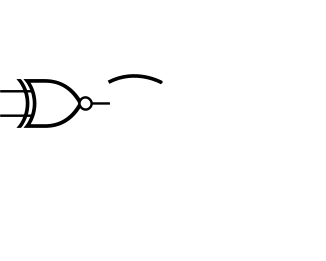
\includegraphics[scale=0.7]{figuras/map-xnor.png}
  \caption{Mapeo de funciones lógicas a celdas estándars}
  \label{fig:map-xnor}
\end{figure}

Es común elegir las celdas estándars según el tipo de aplicación a desarrollar. Existen celdas estandars que fueron diseñadas para bajo consumo, o alta velocidad, o de mínima área. También existe la posibilidad de diseñar celdas que busquen la mejor relación velocidad-consumo-area que puedan ser utilizadas en muchas aplicaciones. En circuitos integrados para sistemas alimentados a batería se intentará utilizar las celdas de menor consumo y evitar siempre que sea posible las de mayor velocidad, en función del presupuesto de potencia disponible para el mismo.

En nuestro caso, seleccionamos una librería de celdas estándars diseñadas para tamaño mínimo de canal n, y p. %Una referencia al Rabaey es necesaria? 
Otra caracteristica de la librería es la distancia entre el riel de VSS hasta el riel VDD. Esta distancia es de 117 lambdas (En nuestra tecnología de 180~nm Lambda es 90nm), lo cual permite el ruteo horizontal de 16 pistas de metal por encima de las celdas, con metal 3 hasta   

 

%http://cmosedu.com/cmos1/electric/electric.htm
% “Tiny-Chip” padframes [1.5 mm x 1.5 mm]

\section{Ubicación y Cableado (\emph{Place \& Route})}
Partimos desde la descripción estructural\footnote{El resultado de la síntesis hecha con lava es un netlist a nivel de compuerta, listo para ser usado por una herramienta de \emph{place \& route}Gate-level netlist vhdl.} del vhdl que producimos en el capítulo \ref{diseñoDigital}. De \emph{Electric} usaremos la herramienta llamada \emph{Silicon Compiler}, que se encarga de ubicar y conectar las celdas según el archivo vhdl. En el apéndice \ref{vhdlNetlist} mostramos el resultado de sintetizar a compuertas nuestro circuito. Las compuertas que se usan son compuertas lógicas genéricas, aún podemos modificar este netlist primero para hacer optimizaciones lógicas, que en nuestro caso esto no es conveniente ya que hemos elegido la arquitectura para lograr la mejor relación de compromiso entre velocidad y menor interconectidad. Otra optimización a realizar es eligiendo la fuerza de la celda.



\emph{place \& route}



Arqu

ero para que este archivo pueda ser usado con Electric fué necesario hacer algunas modificaciones:
\begin{enumerate}
\item Reemplazar los nombres de las instancias de las celdas estandards que  seleccionamos en la sección \ref{celdasEstandars} y \emph{Electric} utilizará.
\item En la parte del vhdl que comienza la descripción estructural es necesario agregar las celdas estandards que serán utilizadas en el circuito.
\item Quitar todas las instancias de \verb|wire port map (...)| volviendo a conectar lo que queda desconectado al quitar estas instancias.
\end{enumerate}  
Estas tareas las realizamos modificando el código del programa de lava que crea el netlist vhdl llamado \verb|VhdlNew.hs|, y con un script\footnote{Adjuntamos el script en el apéndice \ref{scriptPerl}} en perl que es lanzado desde el mismo.
\subsection{}
Una vez que ...

...

%Para simular corners: opConditions.lib



\part{Conclusiones}\label{conclusiones}
	\chapter{Conclusiones finales}
\cursi{Nos hemos propuesto resolver un problema que se encuentra en todos los sistemas de procesamiento de señales y los microprocesadores, lo hemos logrado resolver utilizando herramientas de software libre, y los resultados obtenidos son del orden de magnitud que las soluciones propuestas en otros estudios en la misma tecnología. Para lograr este objetivo, y como subproducto del proceso, en la secciones \ref{subsec:nuevosHDL} y \ref{sec:herramientasDisponibles} brindamos un informe sobre el estado de la cuestión sobre las herramientas de software libre disponibles para el diseño de circuitos integrado.}

  
\section{Metodología}
\paragraph{Gran flexibilidad} Podemos elegir qué herramientas utilizar a lo largo de todo el flujo de diseño. Según la complejidad o magnitud del diseño, hay distintas alternativas. Si en alguna de las etapas del diseño es necesario o preferible utilizar otra herramienta, hemos encontrado que es posible realizarlo gracias a la existencia de formatos estándar para los archivos que utilizan las herramientas de software.



\negrita{Electric} resultó ser la herramienta más simple de instalar y utilizar, y que integra en un único entorno gráfico casi todas las herramientas necesarias para realizar el flujo físico. No incluye herramientas para realizar análisis de performance y potencia, pero utilizando la extracción del \cursi{layout} nos permitió elegir, sin ningún trabajo extra, un simulador analógico (entre varias alternativas posibles) y realizar simulaciones para calcular la potencia y performance. La herramienta de extracción de parásitos de Electric tiene un modelo de parámetros concentrados que realiza una simplificación pesimista. Fué suficiente para realizar el análisis comparativo de las arquitecturas, pero advertimos al lector que existe un camino muy directo y simple para conseguir mejores extracciones de parásitos. Si exportamos el \cursi{layout} en formato \verb.cif. y lo importamos desde Magic, podemos realizar la extracción y el netlist spice para la simulación, ya que la extracción de Magic es mejor que la de Electric y Alliance.

La de extracción de parásitos es realmente crítica, porque será la que nos permita predecir el real funcionamiento de nuestro sistema. La medición de performance y potencia se realizó con \negrita{Gnucap} a partir del \cursi{netlist} spice que genera Electric a partir del \cursi{layout} final. Aunque esta metodología nos permite obtener la mayor presición posible, para circuitos mas grandes empieza a requerir de muchos recursos computacionales. Por ello, existe otra forma de realizar este análisis que se denomina  STA (Static Timing Analisys) que reduce enormemente el esfuerzo de cálculo. Para ello, nuevamente existe una alternativa que se basa en exportar el circuito desde Electric e importarlo en Magic para utilizar su herramienta de STA llamada \verb.vesta..

El \gls{pnr} lo realizamos de forma automática, con la única intervención nuestra para determinar las dimensiones físicas deseadas, en términos de filas y columnas de celdas estándar apiladas.

El HDL (\negrita{Lava}) que hemos utilizado es simplemente un conjunto de módulos de Haskell, por lo tanto realizamos el diseño digital utilizando un único lenguaje de programación de propósito general, aprovechando las ventajas del mismo. Además, hemos realizado la verificación formal de nuestros circuitos, de la misma forma en que describimos los mismos. Cabe mencionar la gran cantidad de alternativas para elegir el HDL, lo cuál permite al diseñador optar por el lenguaje que se ajuste a sus necesidades, con la condición de que tenga la capacidad de producir un \cursi{netlist} VHDL estructural.


También es importante resaltar que esta metodología nos permite realizar \negrita{circuitos secuenciales}. Para ello, a partir del VHDL que nos genera Lava podemos utilizar una herramienta como YOSyS\cite{Yosys} para sintetizar este VHDL comportamental a un netlist a nivel de compuertas. Luego será necesario una traducción desde este \netlist  verilog a un \cursi{netlist} VHDL, si queremos continuar usando Electric. 


\section{Resultados}
Los resultados obtenidos para el sumador de Brent-Kung y Sklansky están en el mismo orden de magnitud que otros estudios\cite{ramanathan,Chatterjee} realizados en 180~\nanom. Considerando que no realizamos iteraciones para mejorar la implementación física, podemos afirmar que hay lugar para optimizar el resultado. Se pueden mejorar los resultados obtenidos por medio de la utilización de otros algoritmos para el \gls{pnr}}. Incluso hay mucho lugar para mejora si personalizamos las celdas estándar para favorecer alguna métrica a costa de otra. Además, si ampliamos nuestro conjunto de celdas estándar a versiones con mayor capacidad de manejo de corriente, sumado a un algoritmo de \gls{pnr} que las utilice allí donde es necesario.

Otra fuente de mejora es realizar el \layout completamente personalizado, sin utilizar herramientas de \gls{pnr}, ya que en baja escala los resultados de un \layout realizado por una persona son más optimos, si entendemos cabalmente el funcionamiento del circuito. Esta última opción sólo será aplicable si la performance de todo el sistema dependiese de éste circuito, porque en general no será posible realizar el layout manualmente ya que lleva mucho más tiempo. Por eso resaltamos que la importancia de estos resultados es que se lograron con una metodología automatizada, lo que nos permite pensar en escalas de circuitos más grande que los sumadores que hemos implementado.

Como conclusión de los resultados obtenidos, podemos afirmar además de lograr un sumador rápido, hemos desarrollado la capacidad de implementar sumadores de cualquier tamaño de forma automática, y que se ajusten a los requerimientos de performance, potencia y área,  según hemos detallado en la sección \ref{subsec:comparativa}.


\section{Aplicaciones}

Con este misma metología queda abierta la posibilidad para la implementación de circuitos combinacionales en general: unidades aritméticas, decodificadores, codificadores, funciones lógicas, etc. 

Para diseñar circuitos secuenciales se requiere algunas tareas y herramientas extras que no hemos utilizado. Se requiere de realizar una síntesis lógica del VDHL que generemos con Lava, y una herramienta de \gls{sta} para chequear las condiciones de \cursi{setup} y \cursi{hold}. Aunque en este trabajo no hemos abordado circuitos de este tipo, hemos mencionado las herramientas necesarias para poder realizarlos, con esta metodología apenas modificada.

También podemos diseñar circuitos analógicos, ya que hemos utilizado tres de las cuatro herramientas básicas para realizarlo: El simulador tipo spice (Gnucap), el editor de \layout y la herramienta de extracción de parásitos. La otra herramienta necesaria es el editor de esquemáticos, pero que está disponible en Electric.

\section{Desafíos futuros}
\begin{itemize}
\item .
\item .
\item .
\end{itemize}




%El hecho de utilizar software libre genera una metodología de trabajo 



\appendix
\chapter{\textsc{ Netlist VHDL }}\label{vhdlNetlist}
\noindent A modo explicativo adjuntamos este archivo generado por Lava.
\begin{lstlisting}
library ieee;

use ieee.std_logic_1164.all;

entity
  BrentKungFastAdder
is
port
  ( 
 
    
    a[0] : in std_logic
  ; a[1] : in std_logic
  ; a[2] : in std_logic
  ; a[3] : in std_logic
  ; a[4] : in std_logic
  ; a[5] : in std_logic
  ; a[6] : in std_logic
  ; a[7] : in std_logic
  ; b[0] : in std_logic
  ; b[1] : in std_logic
  ; b[2] : in std_logic
  ; b[3] : in std_logic
  ; b[4] : in std_logic
  ; b[5] : in std_logic
  ; b[6] : in std_logic
  ; b[7] : in std_logic

  
  ; sum[0] : out std_logic
  ; sum[1] : out std_logic
  ; sum[2] : out std_logic
  ; sum[3] : out std_logic
  ; sum[4] : out std_logic
  ; sum[5] : out std_logic
  ; sum[6] : out std_logic
  ; sum[7] : out std_logic
  ; cout : out std_logic
  );
end BrentKungFastAdder;

architecture
  structural
of
  BrentKungFastAdder
is
  signal w1 : std_logic;
  signal w2 : std_logic;
  signal w3 : std_logic;
  signal w4 : std_logic;
  signal w5 : std_logic;
  signal w6 : std_logic;
  signal w7 : std_logic;
  signal w8 : std_logic;
  signal w9 : std_logic;
  signal w10 : std_logic;
  signal w11 : std_logic;
  signal w12 : std_logic;
  signal w13 : std_logic;
  signal w14 : std_logic;
  signal w15 : std_logic;
  signal w16 : std_logic;
  signal w17 : std_logic;
  signal w18 : std_logic;
  signal w19 : std_logic;
  signal w20 : std_logic;
  signal w21 : std_logic;
  signal w22 : std_logic;
  signal w23 : std_logic;
  signal w24 : std_logic;
  signal w25 : std_logic;
  signal w26 : std_logic;
  signal w27 : std_logic;
  signal w28 : std_logic;
  signal w29 : std_logic;
  signal w30 : std_logic;
  signal w31 : std_logic;
  signal w32 : std_logic;
  signal w33 : std_logic;
  signal w34 : std_logic;
  signal w35 : std_logic;
  signal w36 : std_logic;
  signal w37 : std_logic;
  signal w38 : std_logic;
  signal w39 : std_logic;
  signal w40 : std_logic;
  signal w41 : std_logic;
  signal w42 : std_logic;
  signal w43 : std_logic;
  signal w44 : std_logic;
  signal w45 : std_logic;
  signal w46 : std_logic;
  signal w47 : std_logic;
  signal w48 : std_logic;
  signal w49 : std_logic;
  signal w50 : std_logic;
  signal w51 : std_logic;
  signal w52 : std_logic;
  signal w53 : std_logic;
  signal w54 : std_logic;
  signal w55 : std_logic;
  signal w56 : std_logic;
  signal w57 : std_logic;
  signal w58 : std_logic;
  signal w59 : std_logic;
  signal w60 : std_logic;
  signal w61 : std_logic;
  signal w62 : std_logic;
  signal w63 : std_logic;
  signal w64 : std_logic;
  signal w65 : std_logic;
begin
  c_w2      :  wire  port map (a[0], w2);
  c_w3      :  wire  port map (b[0], w3);
  c_w1      :  xorG  port map (w2, w3, w1);
  c_w6      :  wire  port map (a[1], w6);
  c_w7      :  wire  port map (b[1], w7);
  c_w5      :  xorG  port map (w6, w7, w5);
  c_w8      :  andG  port map (w2, w3, w8);
  c_w4      :  xorG  port map (w5, w8, w4);
  c_w11     :  wire  port map (a[2], w11);
  c_w12     :  wire  port map (b[2], w12);
  c_w10     :  xorG  port map (w11, w12, w10);
  c_w14     :  andG  port map (w6, w7, w14);
  c_w15     :  andG  port map (w5, w8, w15);
  c_w13     :  orG   port map (w14, w15, w13);
  c_w9      :  xorG  port map (w10, w13, w9);
  c_w18     :  wire  port map (a[3], w18);
  c_w19     :  wire  port map (b[3], w19);
  c_w17     :  xorG  port map (w18, w19, w17);
  c_w21     :  andG  port map (w11, w12, w21);
  c_w22     :  andG  port map (w10, w13, w22);
  c_w20     :  orG   port map (w21, w22, w20);
  c_w16     :  xorG  port map (w17, w20, w16);
  c_w25     :  wire  port map (a[4], w25);
  c_w26     :  wire  port map (b[4], w26);
  c_w24     :  xorG  port map (w25, w26, w24);
  c_w29     :  andG  port map (w18, w19, w29);
  c_w30     :  andG  port map (w17, w21, w30);
  c_w28     :  orG   port map (w29, w30, w28);
  c_w32     :  andG  port map (w17, w10, w32);
  c_w31     :  andG  port map (w32, w13, w31);
  c_w27     :  orG   port map (w28, w31, w27);
  c_w23     :  xorG  port map (w24, w27, w23);
  c_w35     :  wire  port map (a[5], w35);
  c_w36     :  wire  port map (b[5], w36);
  c_w34     :  xorG  port map (w35, w36, w34);
  c_w38     :  andG  port map (w25, w26, w38);
  c_w39     :  andG  port map (w24, w27, w39);
  c_w37     :  orG   port map (w38, w39, w37);
  c_w33     :  xorG  port map (w34, w37, w33);
  c_w42     :  wire  port map (a[6], w42);
  c_w43     :  wire  port map (b[6], w43);
  c_w41     :  xorG  port map (w42, w43, w41);
  c_w46     :  andG  port map (w35, w36, w46);
  c_w47     :  andG  port map (w34, w38, w47);
  c_w45     :  orG   port map (w46, w47, w45);
  c_w49     :  andG  port map (w34, w24, w49);
  c_w48     :  andG  port map (w49, w27, w48);
  c_w44     :  orG   port map (w45, w48, w44);
  c_w40     :  xorG  port map (w41, w44, w40);
  c_w52     :  wire  port map (a[7], w52);
  c_w53     :  wire  port map (b[7], w53);
  c_w51     :  xorG  port map (w52, w53, w51);
  c_w55     :  andG  port map (w42, w43, w55);
  c_w56     :  andG  port map (w41, w44, w56);
  c_w54     :  orG   port map (w55, w56, w54);
  c_w50     :  xorG  port map (w51, w54, w50);
  c_w60     :  andG  port map (w52, w53, w60);
  c_w61     :  andG  port map (w51, w55, w61);
  c_w59     :  orG   port map (w60, w61, w59);
  c_w63     :  andG  port map (w51, w41, w63);
  c_w62     :  andG  port map (w63, w45, w62);
  c_w58     :  orG   port map (w59, w62, w58);
  c_w65     :  andG  port map (w63, w49, w65);
  c_w64     :  andG  port map (w65, w27, w64);
  c_w57     :  orG   port map (w58, w64, w57);

  
  c_sum_0   :  wire  port map (w1, sum[0]);
  c_sum_1   :  wire  port map (w4, sum[1]);
  c_sum_2   :  wire  port map (w9, sum[2]);
  c_sum_3   :  wire  port map (w16, sum[3]);
  c_sum_4   :  wire  port map (w23, sum[4]);
  c_sum_5   :  wire  port map (w33, sum[5]);
  c_sum_6   :  wire  port map (w40, sum[6]);
  c_sum_7   :  wire  port map (w50, sum[7]);
  c_cout    :  wire  port map (w57, cout);
end structural;
\end{lstlisting}

\include{Apendice/VhdlNew}
\chapter{\textsc{ Script Perl }}\label{vhdlNetlist}
%\lstset{language=Perl}
\small{
\begin{verbatim}
#!/usr/bin/perl 

#### Import Classes
use File::Copy;
use FileHandle;
####
#### Define constants
my $idPort = "id";

# Input File
my $file =$ARGV[0];

#
my %ports;	# to store ports (ins & outs)
		# and wire's name given
		# by the VhdlNew.hs

### OPEN INPUT FILE 
print "$file\n";
open(my $fhi, '<',$file) or die "archivo no encontrado";
open(my $fho, '+>',"temp-$file");
while(<$fhi>){
#Primero obtengo las entradas
if(m/.+$idPort.+port.map.+\(([A-Za-z0-9_]+).+(w[0-9]+)/)
	{
	push @wires,$2;
	push @wires,$1;
	$ports {$2} = $1;
#	print $fho "--$_"; # comento la linea
	} 

#Ahora obtengo las salidas, por ejemplo:
# c_sum_0   :  std_wire  port map (w1, sum_0);
# o como estas:
# c_cout    :  std_wire  port map (w131, cout);
if(m/.+$idPort.+(w[0-9]+)\,.?([A-Za-z0-9_]+)\).*/)                          
{
$ports {$1} = $2;
print $fho "--$_"; # comento lo que quiero eliminar
} else {
print $fho "$_";}
# and the outputs
#if(m/([a-z]+_[a-z]*_*[0-9]+).+out/) {push @outs,$1;}
# I could use ins and outs to make the %ports hash table
		}#while
close($fhi);
close($fho);


#copy("temp-$file", "temp2-$file");
# Replace all signals connected to wire with the inputs 
#   c_w131    :  std_or2   port map (w132, w141, w131);
# w131 should be replaced by the output


while(my($key,$value) = each(%ports)) {
	open(my $fhi, '<',"temp-$file") or die "archivo no encontrado";
	open(my $fho, '+>', "stripped-$file");
	while(<$fhi>){
		if(s/(.+map.+)$key(\,|\))/$1$value$2/g) {

#need to delete entries with the next pattern:  c_w18     :  std_wire  port map ...
			if(m/.+$idPort.+/) {print $fho "-- deleted $_";}
			else {print $fho "$_";}}
		else { print $fho "$_";}
		      }# while file 

	close($fho);
	close($fhi); #atenti no hacer close($fho, $fhi) porque no es lo mismo que en 2 renglones
	copy("stripped-$file","temp-$file");
					}#while hash table
\end{verbatim}
} %cierra el \small

\chapter{\textsc{ Descripcion en Lava de los sumadores Sklansky y Brent-Kung}}\label{chap:sklansky-lava}
\section{Sumador de Sklansky}
\lstset{language=Haskell} 
\begin{lstlisting}
sklansky :: [(Bit, Bit)] -> ([Bit], Bit)
sklansky abs = (ss,cout)
  where
    gps            = map gpC abs
    (cs,cout)      = (skl (mkFan dotOp) ->- unsnoc ->- (map fst -|- fst) ) gps
    ((_,p) : gps') = gps
    rs             = zip cs gps'
    ss             = p : map sumC rs
--
-- 
{-- La funcion dotOp utilizada es la
 misma que la que definimos para Brent-Kung.

dotOp ((g1, p1) ,(g, p)) = (go, po)
   where
      go = or2 (g, and2 (p, g1))
      po = and2 (p, p1)
--}

{--
Funciones auxiliares utilizadas en el top level de sklanksy:
--}
gpC:: (Bit,Bit) -> (Bit,Bit) -- Genera los g y p a partir de los bit de entrada a y b.
gpC (a,b) = (a <&> b,a <#> b)

sumC :: (Bit,(Bit,Bit)) -> Bit -- Realiza la ultima operacion (una XOR ) para calcular la suma
sumC (cin, (_,p)) = cin <#> p

mkFan :: ((a,a) -> a) -> Fan a
mkFan op (i:is) = i:[op(i,k) | k <- is]

fsT f = (f  -|- id)
snD f = (id -|-  f)

unsnoc as = (init as, last as)
--

-- Red de prefijo de sklansky:
skl :: PP a
skl _ [a] = [a]
skl f as  = init los ++ ros'
  where
    (los,ros) = (skl f las, skl f ras)
    ros'      = f (last los : ros)
    (las,ras) = splitAt (cnd2 (length as)) as

cnd2 n = n - n `div` 2 -- El techo de n/2
--

{--
 Version del sumador que acomoda el tipo de datos de sklansky
 para hacerlo compatible con el modulo para generar el netlist VHDL.
 La version definida arriba toma una lista de tuplas. Y la que 
 creamos aqui toma una tupla de listas:
--}
sklansky_ :: ([Bit], [Bit]) -> ([Bit], Bit) 
sklansky_ (as,bs) = sklansky (zip as bs)
--

\end{lstlisting}


\section{Sumador de Brent-Kung}

\begin{lstlisting}
dotOp ((g1, p1) ,(g, p)) = (go, po)
   where
      go = or2 (g, and2 (p, g1))
      po = and2 (p, p1)
--
unzipl []        = ([],[])
unzipl [a]       = ([a], [])
unzipl (a:b:abs) = (a:as, b:bs)
   where
      (as, bs) = unzipl abs
--
zipl ([], [])     = []
zipl ([a], [])    = []
zipl (a:as, b:bs) = a:b:zipl(as, bs)
--
buf (gin,pin) = (gin, pin)
{-- 
dop toma un operador y un buffer y hace una funcion de 
una lista de duplas a lista de duplas.
Esto es lo que vamos a usar como red de 
prefijo cuando tenemos dos entradas
--}
dop [a,b] = [a, dotOp(a,b)]
--

miti p = unzipl ->- (id -|- p) ->- zipl
--

comb []     = []
comb [a]    = []
comb (a:as) = dop [a, head as]++comb (tail as)
--

posComb (a:as)  = a: (comb (init as))++ [last as]
--
wrapR p = comb ->- miti p ->- posComb 
 
{--
Toda la version del sumador está hecha para que no
 pida como parámetro el dotOp, con esta version no
 se puede usar el programa de Mary para hacer los 
dibujos de las redes, además de perder de vista 
donde se puede poner un buffer real. Esto no es
un gran problema ya que las herramientas de
place & route tienen la capacidad de agregar
o quitar buffers segun sea necesario.
--}
bKung [a] = []
bKung [a, b] = dop [a, b]
bKung as  = wrapR (bKung) as

--
gAndPs ([],[]) = []
gAndPs (a:as, b:bs) = (g,p):gps
   where
      (g, p) = (and2 (a, b),xor2 (a, b))
      gps    = gAndPs (as, bs)
--

fork as = (as, as)
--

evens :: [(Signal Bool,Signal Bool)] -> [Signal Bool]
evens as = cs
   where
      (bs,cs) = unzipp as
--

odds ::  [(Signal Bool,Signal Bool)] -> [Signal Bool]
odds as = bs
   where
      (bs,cs) = unzipp as

--

dropP :: ([Signal Bool], [(Signal Bool,Signal Bool)]) -> ([Signal Bool],[Signal Bool])
dropP = id -|- odds
--

lastXor (as, bs) = map xor2 cs
   where
      cs = zipp (as, bs)
--

sums (a:as, bs) = (a: lastXor (as, init bs),carryOut)
   where
      carryOut = last bs
--

bKungFastAdder = gAndPs ->- fork ->- (evens -|- bKung) ->- dropP ->- sums

\end{lstlisting}

\chapter{\textsc{ Banco de prueba para simulaciones en Gnucap}}\label{chap:gnucap_testbench}
\section{Análisis de potencia de los sumadores}
Estas simulaciones tardaron aproximadamente 10 minutos para los circuitos de 8 bits, 1 hora para los de 16 bits y 14 horas para los circuitos de 32 bits. La computadora en que realizamos las simulaciones tiene 4GB de RAM y las siguientes características detalladas  por el programa \verb.lshw.:
\begin{verbatim}
     *-cpu:0
          description: CPU
          product: Intel(R) Celeron(R) CPU 847 @ 1.10GHz
          vendor: Intel Corp.
          physical id: 41
          bus info: cpu@0
          version: 6.10.7
          serial: 0002-06A7-0000-0000-0000-0000
          slot: SOCKET 0
          size: 800MHz
          capacity: 3800MHz
          width: 64 bits
          clock: 100MHz
    *-cpu:1
          physical id: 1
          bus info: cpu@1
          version: 6.10.7
          serial: 0002-06A7-0000-0000-0000-0000
          size: 800MHz
          capacity: 800MHz
\end{verbatim}

\lstinputlisting{Apendice/tb_potencia.gnucap}
\section{Análisis de performance en los sumadores}

\chapter{\textsc{Scripts para graficar las formas de ondas}}\label{chap:matplotlib}
\noindent Nombre de archivo: \verb_plot.py_, descargar desde \url{http://is.gd/h1aCp6}.
\lstinputlisting[language=Python]{Apendice/plot.py}

\chapter{\textsc{Parámetros de los modelos de simulación}}\label{chap:cmosmodel}
\noindent Descargar este archivo desde \url{http://is.gd/h1aCp6}.
\lstinputlisting{Apendice/tsmc180nm.model}



%\include{Apendice/cmos180nm}

\backmatter


%%%%%%%%%%%%%%%%%% CONFIGURACION DE CABECERA %%%%%%%%%%%%%%%%%%%%%%%%%%%%%%%%%%%%%%
\pagestyle{fancyplain}                                                            %
%%%Formato partes
\renewcommand{\partname}{PARTE}
%%%Formato capítulo: N.Nombre                                                     %
\renewcommand{\chaptermark}[1]{\markboth{\textbf{\small{CAPÍTULO \thechapter}}}{}}%
%%%Formato sección: N.M.Nombre                                                    %
\renewcommand{\sectionmark}[1]{\markright{\textbf{\small{\thesection. #1}}}}      %
%%%%%%%%%%%%%%%%%%%%%%%%%%%%%%%%%%%%%%%%%%%%%%%%%%%%%%%%%%%%%%%%%%%%%%%%%%%%%%%%%%%

\bibliographystyle{classes/CUEDbiblio} % Title is link if provided 
\bibliographystyle{IEEEtran.bst}
\bibliography{biblio}
% Para compilar la primera vez que se agrega una referencia (/cite):
% Seguir estos cuatro pasos:
% latex Nombre-del-archivo.tex
% bibtex Nombre-del-archivo (sin el .tex)
% latex Nombre-del-archivo.tex
% latex Nombre-del-archivo.tex



\end{document}

